\documentclass{article}
\usepackage[utf8]{inputenc}
\usepackage{amsfonts}
% \usepackage{yfonts} % WIP
\usepackage{amsthm}
\usepackage{amsmath}
\usepackage{enumerate}
\usepackage{hyperref}
\usepackage{amssymb}
\usepackage{tikz} % diagram

\begin{filecontents}[overwrite]{commutative-algebra-notes.bib}
@misc{am,
  author = {M. F. Atiyah and I. G. MacDonald},
  title = {{Introduction to Commutative Algebra}},
  year = {1969}
}
@misc{reid,
  author = {Miles Reid},
  title = {{Undergraduate Commutative Algebra}},
  year = {1995}
}
@misc{mit-course,
  author = {Steven Kleiman},
  title = {{Commutative Algebra - MIT OpenCourseWare}},
  year = {2008},
  note = {\url{https://ocw.mit.edu/courses/18-705-commutative-algebra-fall-2008/}},
  url = {https://ocw.mit.edu/courses/18-705-commutative-algebra-fall-2008/}
}
\end{filecontents}
\nocite{*}


\theoremstyle{definition}

\newtheorem{innerdefn}{Definition}
\newenvironment{defn}[1]
{\renewcommand\theinnerdefn{#1}\innerdefn}
{\endinnerdefn}

\newtheorem{innerthm}{Theorem}
\newenvironment{thm}[1]
{\renewcommand\theinnerthm{#1}\innerthm}
{\endinnerthm}

\newtheorem{innerlemma}{Lemma}
\newenvironment{lemma}[1]
{\renewcommand\theinnerlemma{#1}\innerlemma}
{\endinnerlemma}

\newtheorem{innerprop}{Proposition}
\newenvironment{prop}[1]
{\renewcommand\theinnerprop{#1}\innerprop}
{\endinnerprop}

\newtheorem{innercor}{Corollary}
\newenvironment{cor}[1]
{\renewcommand\theinnercor{#1}\innercor}
{\endinnercor}

\newtheorem{innereg}{Example}
\newenvironment{eg}[1]
{\renewcommand\theinnereg{#1}\innereg}
{\endinnereg}

\newtheorem{innerex}{Exercise}
\newenvironment{ex}[1]
{\renewcommand\theinnerex{#1}\innerex}
{\endinnerex}

\newcommand{\aA}{\mathfrak{a}} % TODO: use goth font
\newcommand{\mM}{\mathfrak{m}}

\title{Commutative Algebra notes}
\author{arnaucube}
\date{2026}

\begin{document}

\maketitle

\begin{abstract}
    Notes taken while studying Commutative Algebra, mostly from Atiyah \& MacDonald book \cite{am} and Reid's book \cite{reid}. For the exercises, I follow the assignments listed at \cite{mit-course}.

    Usually while reading books and papers I take handwritten notes in a notebook, this document contains some of them re-written to $LaTeX$.

    The proofs may slightly differ from the ones from the books, since I try to extend them for a deeper understanding.
\end{abstract}

\tableofcontents

\section{Ideals}

\subsection{Definitions}

\begin{defn}{}[ideal]
  $I \subset R$ ($R$ ring) such that $0 \in I$ and $\forall x \in I,~ r \in R,~ xr, rx \in I$.\\
  \hspace*{2em} ie. $I$ absorbs products in $R$.
\end{defn}

\begin{defn}{}[prime ideal]
  if $a, b \in R$ with $ab \in P$ and $P \neq R$ ($P$ a prime ideal), implies $a \in P$ or $b \in P$.
\end{defn}

\begin{defn}{}[principal ideal]
  generated by a single element, $(a)$.

  $(a)$: principal ideal, the set of all multiples $xa$ with $x \in R$.
\end{defn}

\begin{defn}{}[maximal ideal]
  $\mM \subset A$ ($A$ ring) with $m \neq A$ and there is no ideal $I$ strictly between $\mM$ and $A$. ie. if $\mM$ maximal and $\mM \subseteq I \subseteq A$, either $\mM=I$ or $I=A$.
\end{defn}


\begin{defn}{}[unit]
  $x \in A$ such that $xy=1$ for some $y \in A$. ie. element \emph{which divides 1}.
\end{defn}

\begin{cor}{1.8} \label{1.8}
  $A = A^{\times} \sqcup \bigcup m$ (where $\sqcup$ denotes ``disjoint union"), ie. $f \in A$ is either a unit or it is contained in a maximal ideal, not both.
\end{cor}

\begin{defn}{}[zerodivisor]
  $x \in A$ such that $\exists~ 0 \neq y \in A$ such that $xy=0 \in A$. ie. $x$ \emph{divides 0}..


  If a ring does not have zerodivisors is an integral domain.
\end{defn}

\begin{defn}{}[prime spectrum - $Spec(A)$]
  set of prime ideals of $A$. ie.

  $$Spec(A) = \{ P ~|~ P \subset A~ \text{is a prime ideal} \}$$
\end{defn}

\begin{defn}{}[integral domain]
  Ring in which the product of any two nonzero elements is nonzero.

  ie. no zerodivisors.

  ie. $\forall~ 0 \neq a,~ 0 \neq b \in A,~ ab \neq 0 \in A$.

  Every field is an integral domain, not the converse.
\end{defn}

\begin{defn}{}[principal ideal domain - PID]
  integral domain in which every ideal is principal. ie.
  ie. $\forall I \subset R,~ \exists~ a \in I$ such that $I = (a) = \{ ra ~|~ r \in R \}$.
\end{defn}

\begin{defn}{}[nilpotent]
  $a \in A$ such that $a^n=0$ for some $n>0$.
\end{defn}
\begin{defn}{}[nilrad A]
  set of all nilpotent elements of $A$; is an ideal of $A$.

  if $nilrad A = 0 ~\Longrightarrow$ $A$ has no nonzero nilpotents.


  $$nilrad A = \bigcap_{P \in Spec(A)} P$$
\end{defn}

\begin{defn}{}[idempotent]
  $e \in A$ such that $e^2=e$.
\end{defn}

\begin{defn}{}[radical of an ideal]
  $$rad I = \{ f \in A | f^n \in I~ \text{for some}~ n \}$$

  $rad I$ is an ideal.

  $nilrad A = rad 0$

  $rad I = \bigcap_{\substack{P \in \operatorname{Spec}(A)\\ P \supset I}} P$
\end{defn}

\begin{defn}{}[local ring]
  A ring is \emph{local} if it has a unique maximal ideal.

  Notation: local ring $A$, its maximal ideal $\mM$, residue field $K=A/\mM$:
  $$A \supset \mM ~\text{or}~ (A, \mM) ~\text{or}~ (A, \mM, K)$$

  \vspace{0.3cm}
  By Corollary \ref{1.8}, $A$ is local\\
    \hspace*{4em}$\Longleftrightarrow$ $A$ has only one maximal ideal.\\
    \hspace*{4em}$\Longleftrightarrow$ all the nonunits of $A$ form an ideal.
\end{defn}

\subsection{Z and K[X], two Principal Ideal Domains}


\begin{lemma}{}
  $\mathbb{Z}$ is a PID.
\end{lemma}
\begin{proof}
  Let $I$ a nonzero ideal of $\mathbb{Z}$.

  Since $I \neq \{0\}$, there is at least one nonzero integer in $I$. Choose the smallest element of $I$, namely $d$.

  Observe that $(d) \subseteq I$, since $d \in I$. Then, every multiple $nd \in I$, since $I$ is an ideal.

  Take $a \in I$. By the Euclidean division algorithm in $\mathbb{Z}$, $a=qd+r$, with $q,r \in \mathbb{Z}$ and $0 \leq r \leq d$.

  Then $r = a - qd \in I$, but $d$ was chosen to be the smallest positive element of $I$, so the only possibility is $r=0$.

  Hence, $a=qd$, so $a \in (d)$, giving $I \subseteq (d)$.

  Since we had $(d) \subseteq I$ and now we got $I \subseteq (d)$, we have $I = (d)$, so every ideal of $\mathbb{Z}$ is principal. Thus $\mathbb{Z}$ is a Principal Ideal Domain(PID).
\end{proof}

\begin{lemma}{}
  $K[X]$ is a PID.
\end{lemma}
\begin{proof}
  This proof follows very similarly to the previous proof.\\

  Let $K$ be a field, $K[X]$ a polynomial ring.

  Take $\{0\} \neq I \subseteq K[X]$.

  Since $I \neq \{0\}$, there is at least one non-zero polynomial in $I$.

  Let $p(X) \in I$ be of minimal degree among nonzero elements of $I$.

  Observe that $(p(X)) \subseteq I$, because $p(X) \in I$ and $I$ is an ideal.

  Let $f(X) \in I$. By Euclidean division algorithm in $K[X]$, $\exists q, r \in K[X]$ such that $f(X) = q(X) \cdot p(X) + r(X)$ with eithr $r(X)=0$ or $deg(r) < deg(p)$.

  Since $f,p \in I$, then $r(X) = f(X) - q(X)\cdot p(X) \in I$

  If $r(X) \neq 0$, then $deg(r) < deg(p)$, which contradicts the minimality of $deg(p)$ in $I$.

  Therefore, $r(X)=0$, thus $f(X)=q(X)\cdot p(X)$, hence $f(X) \in (p(X))$.
  Henceforth, $I \subseteq (p(X))$.

  Then, since $(p(X)) \subseteq I$ and $I \subseteq (p(X))$, we have that $I = (p(X))$.

  So every ideal of $K[X]$ is principal; thus $K[X]$ is a PID.

\end{proof}



\subsection{Zorn's lemma and Jacobson radicals}

Let $\Sigma$ be a partially orddered set. Given subset $S \subset \Sigma$, an \emph{upper bound} of $S$ is an element $u \in \Sigma$ such that $s<u \forall s \in S$.

A \emph{maximal element} of $\Sigma$, is $m \in \Sigma$ such that $m<s$ does not hold for any $s \in \Sigma$.

A subset $S \subset \Sigma$ is \emph{totally ordered} if for every pair $s_1,s_2 \in S$, either $s_1 \leq s_2$ or $s_2 \leq s_1$.

\begin{lemma}{R.1.7}[Zorn's lemma] \label{zorn}
  Suppose $\Sigma$ a nonempty partially ordered set (ie. we are given a relation $x \leq y$ on $\Sigma$), and that any totally ordered subset $S \subset \Sigma$ has an upper bound in $\Sigma$.

  Then $\Sigma$ has a maximal element.
\end{lemma}

\begin{thm}{AM.1.3} \label{1.3}
  Every ring $A \neq 0$ has at least one maximal ideal.
\end{thm}
\begin{proof}
  By Zorn's lemma \ref{zorn}.
\end{proof}

\begin{cor}{AM.1.4} \label{1.4}
  if $I \neq (1)$ an ideal of $A$, $\exists$ a maximal ideal of $A$ containing $I$.
\end{cor}

\begin{cor}{AM.1.5} \label{1.5}
  Every non-unit of $A$ is contained in a maximal ideal.
\end{cor}

\begin{defn}{}[Jacobson radical]
  The \emph{Jacobson radical} of a ring $A$ is the intersection of all the maximal ideals of $A$.

  Denoted $Jac(A)$.
  
  $Jac(A)$ is an ideal of $A$.
\end{defn}

\begin{prop}{AM.1.9} \label{1.9}
  $x \in Jac(A)$ iff $(1 - xy)$ is a unit in $A$, $\forall y \in A$.
\end{prop}
\begin{proof}
  Suppose $1-xy$ not a unit.

  By \ref{1.5}, $1-xy \in \mM$ for $\mM$ some maximal ideal.

  But $x \in Jac(A) \subseteq \mM$, since $Jac(A)$ is the intersection of all maximal ideals of $A$.

  Hence $xy \in \mM$, and therefore $1 \in \mM$, which is absurd, thus $1-xy$ is a unit.

  Conversely:\\
  Suppose $x \not\in \mM$ for some maximal ideal $\mM$.

  Then $\mM$ and $x$ generate the unit ideal $(1)$, so that we have $u + xy = 1$ for some $u \in \mM$ and some $y \in A$.

  Hence $1 -xy \in \mM$, and is therefore not a unit.
\end{proof}

\section{Modules}

\subsection{Modules concepts}

Let $A$ be a ring. An $A$-module is an Abelian group $M$ with a multiplication
map
\begin{align*}
  A \times M &\longrightarrow M\\
  (f, m) &\longmapsto fm
\end{align*}
satisfying $\forall~ f,g \in A,~~ m, n \in M$.
\begin{enumerate}[i.]
  \item $f(m \pm n)=fm \pm fn$
  \item $(f \pm g) m = fm \pm gm$
  \item $(fg) m = f(gm)$
  \item $1_A m = m$
\end{enumerate}

Let $\psi: M \longrightarrow M$ an $A$-linear endomorphism of $M$.\\
$A[\psi] \subset End M$ is the subring geneerated by $A$ and the action of $\psi$.
\begin{itemize}
\item since $\psi$ is $A$-linear, $A[\psi]$ is a commutative ring.
\item $M$ is a module over $A[\psi]$, so $\psi$ beomes multiplication by a ring element.
\end{itemize}

\subsection{Cayley-Hamilton theorem, Nakayama lemma, and corollaries}

\begin{prop}{AM.2.4}(Cayley-Hamilton Theorem) \label{2.4}
  Let $M$ a fingen $A$-module. Let $\aA$ an ideal of $A$, let $\psi$ an
  $A$-module endomorphism of $M$ such that $\psi(M) \subseteq \aA M$.

  Then $\psi$ satisfies
  
  $$\psi^n + a_1 \psi^{n-1} + \ldots + a_{n-1} \psi + a_n = 0$$

  with $a_i \in \aA$.
\end{prop}
\begin{proof}
  Since $M$ fingen, let $\{ x_1, \ldots, x_n \}$ be generators of $M$.\\
  By hypothesis, $\psi(M) \subseteq \aA M$; so for any generator $x_i$, it's image $\psi(x_i) \in \aA M$.

  Any element in $\aA M$ is a linear combination of the generators with coefficients in the ideal $\aA$, thus
  $$\psi(x_i)= \sum_{j=1}^n a_{ij} x_j$$
  with $a_{ij} \in \aA$.
  
  Thus, for a module with $n$ generators, we have $n$ different $\psi(x_i)$ equations:

  $$
  \left.
  \begin{aligned}
    \psi(x_1) &= a_{1,1} x_1 + a_{1,2} x_2 + \ldots + a_{1,n} x_n\\
    \psi(x_2) &= a_{2,1} x_1 + a_{2,2} x_2 + \ldots + a_{2,n} x_n\\
    \ldots\\
    \psi(x_n) &= a_{n,1} x_1 + a_{n,2} x_2 + \ldots + a_{n,n} x_n
  \end{aligned}
  \right\}
  \begin{aligned}
      &\text{n elements $\psi(x_i) \in \aA M$ which}\\
      &\text{are linear combinations of the}\\
      &\text{$n$ generators of $M$}
  \end{aligned}
  $$
  
  Next step: rearrange in order to use matrix algebra.

  Observe that each row equals $0$, and rearranging the elements at each row we get

  $$
  \left.
  \begin{aligned}
    &\psi(x_1) - (a_{1,1} x_1 + a_{1,2} x_2 + \ldots + a_{1,n} x_n) = 0\\
    &\psi(x_2) - (a_{2,1} x_1 + a_{2,2} x_2 + \ldots + a_{2,n} x_n) = 0\\
    &\ldots\\
    &\psi(x_n) - (a_{n,1} x_1 + a_{n,2} x_2 + \ldots + a_{n,n} x_n) = 0
  \end{aligned}
  \right\}
  $$

  Then, group the $x_i$ terms together; as example, take the row $i=1$:
    $$(\psi - a_{1,1})x_1 - a_{1,2} x_2 - \ldots - a_{1,n} x_n = 0$$

  $$
  \left.
  \begin{aligned}
    &~~~~(\psi - a_{1,1})x_1 - a_{1,2} x_2 - \ldots - a_{1,n} x_n = 0\\
    &-a_{2,1} x_1 + (\psi - a_{2,2}) x_2 - \ldots - a_{2,n} x_n = 0\\
    &\ldots\\
    &-a_{1,1} x_1 - a_{1,2} x_2 - \ldots + (\psi - a_{1,n}) x_n = 0\\
  \end{aligned}
  \right\}
  $$
    
  So, $\forall i \in [n]$, as a matrix:
  
  $$
  \begin{pmatrix}
    \psi - a_{1,1} & -a_{1,2} & \ldots & -a_{1,n}\\
    -a_{2,1} & \psi-a_{2,2} & \ldots & -a_{2,n}\\
    \vdots\\
    -a_{n,1} & -a_{n,2} & \ldots & \psi-a_{n,n}\\
  \end{pmatrix}
  \begin{pmatrix}
    x_1\\ x_2\\ \vdots\\ x_n
  \end{pmatrix}
  =
  \begin{pmatrix}
    0\\ 0\\ \vdots\\ 0
  \end{pmatrix}
  $$


  
  Denote the previous matrix by $\Phi$. Let $m$ denote the vector $(x_1, x_2, \ldots, x_n)^T$ (ie. the vector of generators of the $A$-module $M$).\\
  \hspace*{4em}Then we can write the previous equality as
  \begin{equation}
    \Phi \cdot m = 0
    \label{eq:2.4.1}
  \end{equation}

  We know that
  \begin{equation}
    adj(\Phi) \Phi = det(\Phi) I
    \label{eq:2.4.2}
  \end{equation}
  (aka. \emph{fundamental identity for the adjugate matrix}).

  So if at \eqref{eq:2.4.1} we multiply both sides by $adj(\Phi)$,
  \begin{align*}
    adj(\Phi) \cdot \Phi \cdot &m = 0\\
    (\text{recall from \eqref{eq:2.4.2}:}~ &adj(\Phi)\Phi=det(\Phi)\cdot I ~)\\
    =det(\Phi) \cdot I \cdot &m = 0
  \end{align*}

  Thus,
  \begin{align*}
    det(\Phi) \cdot I \cdot &m = 0:\\
  \begin{pmatrix}
    det(\Phi) & 0 & \ldots & 0\\
    0 & det(\Phi) & \ldots & 0\\
    \vdots\\
    0 & 0 & \ldots & det(\Phi)
  \end{pmatrix}
  \cdot
  &\begin{pmatrix}
    x_1\\ x_2\\ \vdots\\ x_n
  \end{pmatrix}
                              =
  \begin{pmatrix}
    0\\ 0\\ \vdots\\ 0
  \end{pmatrix}
  \end{align*}

  $\Longrightarrow$
  \begin{equation}
    det(\Phi) \cdot x_i = 0 ~~\forall i \in [n]
    \label{eq:2.4.3}
  \end{equation}

  ie. $det(\Phi)$ is an \emph{annihilator} of the generators $x_i$ of $M$, thus
  is an annihilator of the entire module $M$.


  So, we're interested into calculating the $det(\Phi)$.

  By the Leibniz formula,
  $$\det(A) = \sum_{\sigma \in S_n} sgn(\sigma) \prod_{i=1}^n a_{i, \sigma(i)}$$

  thus,
  $$det(\Phi) = \underbrace{(\psi - a_{11}) (\psi - a_{22}) \ldots (\psi - a_{nn})}_{\text{diagonal of $\Phi$, leading term of the determinant}} - \ldots$$

  The \emph{determinant trick} is that the terms that go after the "leading term of the determinant", will belong to $\aA$ and their combinations with $\psi$ will not be bigger than $\psi^n$. Furthermore, when expanding it
  \begin{itemize}
    \item highest power is $1 \cdot \psi^n$
    \item coefficient of $\psi^{n-1}$ is $-( \underbrace{ a_{11} + a_{22} + \ldots + a_{nn} }_{a_1})$,\\
      where, since each $a_{ii} \in \aA,~~ a_1 \in \aA$
    \item the rest of coefficients of $\psi^k$ are also elements in $\aA$
  \end{itemize}

  Therefore we have
  $$det(\Phi) = \psi^n + a_1 \psi^{n-1} + a_2 \psi^{n-2} + \ldots + a_{n-1} \psi + a_n$$
  with $a_i \in \aA$.

  \vspace{0.5cm}

  Now, notice that we had $det(\Phi) \cdot x_i = 0 ~\forall~ i\in [n]$.

  The matrix $\Phi$ is the \emph{characteristic matrix}, $xI-A$, viewed as an operator. Then,
  $$det(\Phi) = det(xI-A) = p(x)$$
  where $p(x)$ is the \emph{characteristic polynomial}.

  If a linear transformation turns every basis vector ($x_i$) into zero, then that transformation is the zero transformation. So in our case, $det(\Phi)$ is the zero transformation, thus $det(\Phi)=0$.
  Therefore,
  $$\psi^n + a_1 \psi^{n-1} + a_2 \psi^{n-2} + \ldots + a_{n-1} \psi + a_n = 0$$


  %%%%%% OLD START

  % \vspace{3cm}
  % 
  % Kronecker delta:
  % $\delta_{ij} =
  % \begin{cases}
  %   1 & \text{if } i = j,\\
  %   0 & \text{otherwise}
  % \end{cases}$
  % 
  % With the Kronecker delta, $\psi(x_i)$ can be expressed as
  % $$\psi(x_i) = \sum_{j=1}^n \delta_{ij} \psi(x_j)$$
  % so the previous matrix can be characterized as
  % $$\sum_{j=1}^n (\delta_{ij} \psi - a_{ij}) x_j = 0$$
  % 
  % The entries of the matrix are \emph{endomorphisms} (elements of the ring $A[\psi]$)
  % \begin{itemize}
  %   \item the term $(\psi - a_{11})$ is an operator that acts on $x_1$; as $(\psi(x_1)-a_{11}\cdot x_1)$
  %   \item the term $(-a_{12})$ is an operator that acts on $x_2$; as multiplication by it, ie. $(-a_{12} \cdot x_2)$
  % \end{itemize}
  % 
  % We need a single element $x \in A$ that \emph{annihilates} every $m \in M$ simultaneously, ie. $xM=0$. We're going to use the determinant for getting $x$.
  % 
  % Since $A$ is a commutative ring, and $\psi$ commutes with any $a \in A$,
  % the ring of operators $A[\psi]$ is a commutative ring.
  % 
  % $\Longrightarrow~$ so we can treat the matrix as a matrix of real numbers and calculate its determinant.
  % 
  % 
  % \vspace{0.75cm}
  % This is called \emph{"the determinant trick"}.\\
  % We're interested in the determinant because it is the only way to turn a system of multiple equations in a single scalar-like equation that describes the endomorphism $\psi$.\\
  % $\rightarrow$ Because in module theory, we lack of "division", so can not "solve for $\psi$" the system of equations.\\
  % $\rightarrow$ The determinant provides a way to find a polynomial that \emph{annihilates} the module; the \emph{characteristic polynomial}, which related $\psi$ to the ideal $\aA$
  % 
  % $$det(M) \cdot x_i = 0~~ \forall i$$
  % where $x_i$ are the generators of $M$.
  % 
  % Use $\Phi$ to denote the previous matrix. The determinant is the only function that can take that matrix $\Phi$ and produce a single scalar $x=det(\Phi)$ such that the following identity holds: $adj(\Phi)\cdot \Phi=det(\Phi) \cdot \aA$.
  % \vspace{0.5cm}
  % 
  % Since $det(M)$ kills every generator, it must kill every element in $M$\\
  % $\Longrightarrow~~ det(M)$ is the zero map.
  % 
  % Leibniz formula of the determinant of an $n \times n$ matrix:
  % $$
  % det(M) = \sum_{\sigma \in S_n} sign(\sigma) \prod_{i=1}^n M_{i, \sigma(i)}
  % $$
  % 
  % so,
  % $$(\psi - a_{11}) (\psi - a_{22}) \ldots (\psi - a_{nn})$$
  % expanding it,
  % \begin{itemize}
  %   \item highest power is $1 \cdot \psi^n$
  %   \item coefficient of $\psi^{n-1}$ is $-( \underbrace{ a_{11} + a_{22} + \ldots + a_{nn} }_{a_1})$,\\
  %     where, since each $a_{ii} \in \aA,~~ a_1 \in \aA$
  %   \item the rest of coefficients of $\psi^k$ are also elements in $\aA$
  % \end{itemize}
  % 
  % So we have
  % $$p(\psi) = \psi^n + a_1 \psi^{n-1} + a_2 \psi^{n-2} + \ldots + a_{n-1} \psi + a_n$$
  % with $a_i \in \aA$.
  % 
  % Since this determinant annihilates the generators (ie. $det(M)x_i=0$), the resulting enddomorphism $p(\psi)$ is the zero map on the entire module $M$, so:
  % $$\psi^n + a_1 \psi^{n-1} + a_2 \psi^{n-2} + \ldots + a_{n-1} \psi + a_n = 0$$
  % with $a_i \in \aA$, as stated in the Cayley-Hamilton theorem.
  
  %%%%% OLD END
\end{proof}


\vspace{0.5cm}

\begin{cor}{AM.2.5} \label{2.5}
  Let $M$ a fingen $A$-module, let $\aA$ an ideal of $A$ such that $\aA M = M$.

  Then, $\exists~ x \equiv 1 \pmod \aA$ such that $xM = 0$.
\end{cor}
\begin{proof}
  take $\psi = \text{identity}$. Then in Cayley-Hamilton (\ref{2.4}):
  \begin{align*}
    &\psi^n + a_1 \psi^{n-1} + a_2 \psi^{n-2} + \ldots + a_{n-1} \psi + a_n = 0\\
    \Longrightarrow~ &id_M + a_1 id_M + a_2 id_M + \ldots + a_{n-1} id_M + a_n = 0\\
    \Longrightarrow~ &(1 + a_1 + \ldots + a_n) id_M = 0
  \end{align*}
  apply it to $m \in M$, where since $id_M(m)=m$ (by definition of the identity), we then have
  $$(1 + a_1 + \ldots + a_n) \cdot m = 0$$
  with $a_i \in \aA$.

  \begin{enumerate}[\text{part} i.]
    \item $xM=0$:\\
      Thus the scalar $x = (1 + a_1 + \ldots + a_n)$ annihilates every $m \in M$, ie. the entire module $M$.

    \item $x \equiv 1 \pmod \aA$:\\
      $x \equiv 1 \pmod \aA ~~ \Longleftrightarrow (x-1) \in \aA$\\
      then from $x = (1 + \underbrace{a_1 + \ldots + a_n}_b) \in \aA$, set $b=a_1 + \ldots + a_n$,\\
      so that $x=(1+b) \in \aA$.\\

      Then $x-1 = (1+b)-1 = b \in \aA$\\
      so $x-1 \in \aA$, thus $x \equiv 1 \pmod \aA$ as stated.
  \end{enumerate}
\end{proof}



\begin{prop}{AM.2.6}[Nakayama's lemma] \label{2.6}
  Let $M$ a fingen $A$-module, let $\aA$ an ideal of $A$ such that $\aA \subseteq Jac(A)$.

  Then $\aA M = M$ implies $M=0$.
\end{prop}
\begin{proof}
  By \ref{2.5}: since $\aA M = M$, we have $x M =0$ for some $x \equiv 1 \pmod {Jac(A)}$. (notice that at \ref{2.5} is $\pmod \aA$ but here we use $\pmod {Jac(A)}$, since we have $\aA \subseteq Jac(A)$).

  (recall \ref{1.9}: $x \in Jac(A)$ iff $(1 - xy)$ is a unit in $A$, $\forall y \in A$).\\
  By \ref{1.9}, $x$ is a unit in $A$ (thus $x^{-1}\cdot x=1$).

  Hence $M = x^{-1} \cdot \underbrace{x~ \cdot M}_{=0~ \text{(by \ref{2.5})}} = 0$.

  Thus, if $\aA M = M$ then $M=0$.
\end{proof}



\begin{cor}{AM.2.7} \label{2.7}
  Let $M$ a fingen $A$-module, let $N \subseteq M$ a submodule of $M$, let $\aA \subseteq Jac(A)$ an ideal.

  Then $M = \aA M + N \stackrel{\text{implies}}{\Longrightarrow} M=N$.
\end{cor}
\begin{proof}
  The idea is to apply Nakayama (\ref{2.6}) to $M/N$.

  Since $M$ fingen $\Longrightarrow~~ M/N$ is fingen and an $A$-module.

  Since $\aA \subseteq Jac(A) ~\Longrightarrow~$ Nakayama applies to $M/N$ too.

  By definition,
  $$\aA M = \left\{ \sum a_i \cdot m_i ~~|~~ a_i \in \aA, m_i \in M \right\}$$
  where $m_i$ are the generators of $M$.

  Then, for $M/N$,
  $$\aA (\frac{M}{N}) = \left\{ \sum a_i \cdot (m_i + N) ~~|~~ a_i \in \aA, m_i \in M \right\}$$

  observe that $a_i(m_i+N)= a_i m_i +N$, thus
  $$\sum_i a_i \cdot (m_i + N) = \underbrace{(\sum_i a_i \cdot m_i)}_{\in \aA M} + N \in \aA M + N$$

  Hence,

  \begin{equation}
    \aA (\frac{M}{N}) = \left\{ x + N ~~|~~ x \in \aA M \right\} = \aA M + N
    \label{eq:2.7.1}
  \end{equation}

  By definition, if we take $\frac{\aA M + N}{N}$, then
  $$\frac{\aA M + N}{N} = \left\{ y + N ~~|~~ y \in \aA M +N \right\} = \aA M + N$$

  thus every $y \in \aA M +N$ can be written as
  $$y=x+n,~~ \text{with}~ x \in \aA M,~ n\in N$$
  which comes from \eqref{eq:2.7.1}.

  Thus, $y + N = (x+n)+N = x+N$, since $n \in N$ is zero in the quotient.
  
  Hence, every element of $\frac{\aA M +N}{N}$ has the form
  $$\frac{\aA M + N}{N} = \left\{ x + N ~~|~~ x \in \aA M \right\}$$
  as in \eqref{eq:2.7.1}.

  Thus
  \begin{equation}
    \aA (\frac{M}{N}) = \aA M + N = \frac{\aA M +N}{N}
    \label{eq:2.7.2}
  \end{equation}

  By the Collorary assumption, $M = \aA M + N$; quotient it by $N$:
  \begin{equation}
    \frac{M}{N} = \frac{\aA M +N}{N}
  \label{eq:2.7.3}
  \end{equation}

  So, from \eqref{eq:2.7.2} and \eqref{eq:2.7.3}:
  $$\aA (\frac{M}{N}) = \aA M +N = \frac{\aA M +N}{N} = \frac{M}{N}$$
  thus, $\aA (\frac{M}{N}) = \frac{M}{N}$.

  By Nakayama's lemma \ref{2.6}, if $\aA (\frac{M}{N}) = \frac{M}{N} ~\stackrel{implies}{\Longrightarrow}~ \frac{M}{N}=0$

  Note that
  $$\frac{M}{N} = \{ m + N ~|~ m \in M \}$$
  (the zero element in $\frac{M}{N}$ is the coset $N=0+N$)

  Then, $\frac{M}{N}=0$ means that the quotient has exactly one element, the zero coset $N$.

  Thus, every coset $m + N$ equals the zero coset $N$, so $m-0 \in N ~\Longrightarrow~ m \in N$.

  Hence every $m \in M$ lies in $N$, ie. $\forall m \in M,~ m \in N$.

  So $M \subseteq N$. But notice that by the Corollary, we had $N \subseteq M$, therefore $M = N$.

  Thus, if $M = \aA M + N \stackrel{implies}{\Longrightarrow} M = N$.
\end{proof}



\begin{prop}{AM.2.8} \label{2.8}
  Let $x_i ~\forall i \in [n]$ be elements of $M$ whose images $\frac{M}{m M}$ from a basis of this vector space. Then the $x_i$ generate $M$.
\end{prop}
\begin{proof}
  Let $N$ submodule $M$, generated by the $x_i$.

  Then the composite map $N \longrightarrow M \longrightarrow \frac{M}{m M}$ maps $N$ onto $\frac{M}{m M}$, hence $N + \aA M = M$, which by \ref{2.7} implies $N = M$.
\end{proof}


\subsection{Sequences}

\begin{defn}{R.2.9.a}[Exact Sequence]
  Let a sequence of homomorphisms
$$L \stackrel{\alpha}{\longrightarrow} M \stackrel{\beta}{\longrightarrow} N$$
It is \emph{exact} at $M$ if $im(\alpha)=ker(\beta)$.

ie. $\beta \circ \alpha = 0$ and $\alpha$ maps surjectively to
$ker(\beta)$.
\end{defn}

\begin{defn}{R.2.9.b}[Short Exact Sequence (s.e.s.)] \label{2.9}
$$0 \longrightarrow L \stackrel{\alpha}{\longrightarrow} M \stackrel{\beta}{\longrightarrow} N \longrightarrow 0$$
is exact $\Longleftrightarrow~ L \subset M$ and $N=M / L$.

Properties:
\begin{itemize}
  \item $\alpha$ injective
  \item $\beta$ surjective
  \item $\alpha:~ L \Longrightarrow ker \beta$
  \item $\beta$ induces $M/\alpha(L) \longrightarrow N$
\end{itemize}
\end{defn}

\begin{prop}{R.2.10}[Split exact sequence] \label{2.10}
  For the previous s.e.s., 3 equivalent conditions:
  \begin{enumerate}[i.]
    \item $\exists$ isomorphism $M \cong L \oplus N$, with
      \begin{align*}
        \alpha:~ &m \longmapsto (m,0)\\
        \beta:~ &(m, n) \longmapsto n
      \end{align*}

    \item $\exists$ a \emph{section} of $\beta$, that is, a map $s: N \longrightarrow M$ such that $\beta \circ s = id_N$
    \item $\exists$ a \emph{retraction} of $\alpha$, that is, a map $r: M \longrightarrow L$ such that $r \circ \alpha = id_L$
  \end{enumerate}
  
  If all i, ii, iii are satisfied, it is a split exact sequence.
\end{prop}
\begin{proof}
  Intuitively, when a s.e.s. \emph{splits} it means that the middle module $M$ is the direct sum of the other (outer) two modules, ie. $M = L \oplus N$.

  \begin{itemize}
    \item[(i to ii, iii)]
      if $M \cong L \oplus N$ such that $\alpha:~ m \longmapsto (m,0),~~ \beta:~ s(m, n) \longmapsto n$, we can define the maps

      for ii:
      \begin{align*}
        s:~ N &\longrightarrow L \oplus N\\
        s(n) &\longmapsto (0, n)
      \end{align*}

      Then $\beta(s(n))=\beta(0,n)$, so $\beta \circ s = id_N$.

      for iii:
      \begin{align*}
        r:~ L \oplus N &\longrightarrow L\\
        r(m,n) &\longmapsto m
      \end{align*}

      Then $r(\alpha(m))=r(m,0)$, so $r \circ \alpha = id_L$.

    \item[(ii to i)]
      assume $s: N \longrightarrow M$ such that $\beta \circ s = id_M$

      Want to show $M \cong im(\alpha) \oplus im(s)$.

      $\forall m \in M$, consider $m - s(\beta(m))$, apply $\beta$ to it:\\
      $\beta(m - s(\beta(m))) = \beta(m) - (\beta \circ s)(\beta(m)) = \beta(m) - \beta(m) = 0$

      Since $ker(\beta) = im(\alpha),~~ \exists! l \in L ~\text{such that}~ \alpha(l) = m - s(\beta(m))$.

      Thus $m = \alpha(l) + s(\beta(m))$.

      \vspace{0.3cm}
      Now, suppose $x \in im(\alpha) \cap im(s)$, then $x = \alpha(l)=s(n)$, apply $\beta$ to it: $\beta(\alpha(l)) = \beta(s(n)) ~\Longrightarrow~ 0=n$.

      If $n=0$, then $s(n)=0$, so the intersection is $\{0\}$.

      \vspace{0.3cm}
      Define
      \begin{align*}
        \phi: L \oplus N &\longrightarrow M\\
        \phi(l,n) &\longmapsto \alpha(l)+s(n)
      \end{align*}
      This isomorphism satisfies the required conditions.

    \item[(iii to i)] similar to the previous one.
  \end{itemize}

  \vspace{0.3cm}
  Overview:\\

$$
0 \longrightarrow L
  \substack{
    \stackrel{\alpha}{\longrightarrow}\\
    \stackrel{\longleftarrow}{r}
  }
  \substack{M \\[0.5ex] \cong L \oplus N}
  \substack{
    \stackrel{\beta}{\longrightarrow}\\
    \stackrel{\longleftarrow}{s}
  }
  N \longrightarrow 0
$$
\begin{align*}
  \alpha:~ &l \longmapsto (l,0)\\
  r:~ &(m,n) \longmapsto m\\
  \alpha &\circ r = id_L\\
  \beta:~ &(l,n) \longmapsto n\\
  s:~ &n \longmapsto (0,n)\\
  \beta &\circ s = id_N
\end{align*}

\end{proof}

\section{Noetherian rings (and modules)}

\begin{defn}{}[Ascending Chain Condition]
  A partially orddered set $\Sigma$ has the \emph{ascending chain condition} (a.c.c.) if every chain
  $$s_1 \leq s_2 \leq \ldots \leq s_k \leq \ldots$$
  eventually breaks off, that is, $s_k = s_{k+1} = \ldots$ for some $k$.
\end{defn}

$\Longrightarrow~ \Sigma$ has the a.c.c. iff every non-empty subset $S \subset \Sigma$ has a maximal element.\\
\hspace*{2em} if $\empty \neq S \subset \Sigma$ does not have a maximal element, choose $s_1 \in S$, and for each $s_k$, an element $s_{k+1}$ with $s_k < s_{k+1}$, thus contradicting the a.c.c.

\subsection{Noetherian rings and modules}
\begin{defn}{R.3.2}[Noetherian ring]\\
  Let $A$ a ring; 3 equivalent conditions:
  \begin{enumerate}[i.]
    \item the set $\Sigma$ of ideals of $A$ has the a.c.c.; in other words, every increasing chain of ideals
      $$I_1 \subset I_2 \subset \ldots \subset I_k \subset \ldots$$
      eventually stops, that is $I_k = I_{k+1}=\ldots$ for some $k$.
    \item every nonempty set $S$ of ideals has a maximal element
    \item every ideal $I \subset A$ is finitely generated
  \end{enumerate}
  If these conditions hold, then $A$ is \emph{Noetherian}.
\end{defn}
\begin{proof}
  TODO
\end{proof}

\begin{defn}{R.3.4.D}[Noetherian modules]\\
  An $A$-module $M$ is Noetherian if the submoles of $M$ have the a.c.c.,\\
  that is, ay increasing chain
  $$M_1 \subset M_2 \subset \ldots \subset M_k \subset \ldots$$
  of submodules eventually stops.
\end{defn}

As in with rings, it is equivalent to say that
\begin{enumerate}[i.]
  \item any nonempty set of modulesof $M$ has a maximal element
  \item every submodule of $M$ is finite
\end{enumerate}



\begin{prop}{R.3.4.P}\label{R.3.4.P}
  Let $0 \longrightarrow L \xrightarrow{\ \alpha \ } M \xrightarrow{\ \beta \ } N \longrightarrow 0$ be a s.e.s. (split exact sequence, \ref{2.10}).

  Then, $M$ is Noetherian $\Longleftrightarrow~ L$ and $N$ are Noetherian.
\end{prop}
\begin{proof}
  $\Longrightarrow$: trivial, since ascending chains of submodules in $L$ and $N$ correspond one-to-one to certain chains in $M$.

  $\Longleftarrow$: suppose $M_1 \subset M_2 \subset \ldots \subset M_k \subset \ldots$ is an increasing chain of submodules of $M$.

  Then identifying $\alpha(L)$ with $L$ and taking intersection gives a chain
  $$L \cap M_1 \subset L \cap M_2 \subset \ldots \subset L \cap M_k \subset \ldots$$
  of submodules of $L$, and applying $\beta$ gives a chain
  $$\beta(M_1) \subset \beta(M_2) \subset \ldots \beta(M_k) \subset \ldots$$
  of submodules of $N$.

  Each of these two chains eventually stop, by the assumption on $L$ and $N$, so that we only need to prove the following lemma which completes the proof.
\end{proof}

\begin{lemma}{R.3.4.L}
  for submodules $M_1 \subset M_2 \subset M$,
  $$L \cap M_1 = L \cap M_2 ~\text{and}~ \beta(M_1) = \beta(M_2) ~\Longrightarrow~ M_1 = M_2$$
\end{lemma}
\begin{proof}
  if $m\in M_2$, then $\beta(m) \in \beta(M_1) = \beta(M_2)$, so that there is an $n \in M_1$ such that $\beta(m)=\beta(n)$.

  Then $\beta(m-n)=0$, so that
  $$m - n \in M_2 \cap ker(\beta)=M_1 \cap ker(\beta)$$

  Hence $m \in M_1$, thus $M_1 = M_2$.
\end{proof}



\begin{cor}{R.3.5}[Properties of Noetherian modules]\label{R.3.5}
  \begin{enumerate}[i.]
    \item if $\forall i \in [r],~~M_i$ are Noetherian modules, then
      $\bigoplus_{i=1}^r M_i$ is Noetherian.
    \item if $A$ a Noetherian ring, then an $A$-module $M$ is Noetherian iff it is finite over $A$.
    \item if $A$ a Noetherian ring, $M$ a finite module, then any submodule $N \subset M$ is again finite.
    \item if $A$ a Noetherian ring, and $\psi: A \longrightarrow B$ a ring homomorphism such that $B$ is a finite $A$-module, then $B$ is a Noetherian ring.
  \end{enumerate}
\end{cor}
\begin{proof}
  \begin{enumerate}[i.]
    \item a direct sum $M_1 \oplus M_2$ is a particular case of an exact sequence.

      Then, Proposition \ref{R.3.4.P} proves this statement when $r=2$. The case $r>2$ follows by induction.

    \item if $M$ finite, then $\exists~$ surjective homomorphism
      $$A^r \longrightarrow M \longrightarrow 0$$
      for some $r$, so that $M$ is a quotient
      $$M \cong A^r / N$$
      for some submodule $N \subset A^r$.

      $A^r$ is a Noetherian module by i., so $M$ is Noetherian due Proposition \ref{R.3.4.P}.

      Conversely, $M$ Noetherian implies $M$ finite.
      
      item as in previous implications:\\
      $M$ finite and $A$ Noetherian $\Longrightarrow$ $M$ is Noetherian,\\
      $\Longrightarrow$ since $N \subseteq M$, then $N$ is Noetherian too\\
      $\Longrightarrow$ which implies that $N$ is a finite $A$-module.

    \item $B$ is Noetherian as an $A$-module; but ideals of $B$ are submodules of $B$ as an $A$-submodule, so that $B$ is a Noetherian ring.
  \end{enumerate}
\end{proof}


\vspace{0.5cm}
\subsection{Hilbert basis}
\begin{thm}{R.3.6}[Hilbert basis theorem] \label{hilbert-basis}
  If $A$ a Noetherian ring, then so is the polynomial ring $A[x]$.
\end{thm}
\begin{proof}
  Prove that any ideal $I \subset A[x]$ is fingen.

  Define auxiliary sets $J_n \subset A$ by
  $$J_n = \{ a \in A ~|~ \exists f \in I ~\text{s.th.}~ f = a x^n + b_{n-1}x^{n-1} + \ldots b_0 \}$$
  ie. $J_n$ is the set of leading coefficients of $I$ of degree $n$.

  $J_n$ is an ideal, since $I$ is an ideal.

  $J_n \subset J_{n+1}$, since for $f \in I$ also $x f \in I$.

  Therefore $J_1 \subset J_2 \subset \ldots \subset J_k \subset \ldots$ is an increasing chain of ideals.\\
  Using the assumption that $A$ is Noetherian, deduce that $J_n = J_{n+1}$ for some $n$.

  For each $m \leq n, ~~ J_m \subset A$ is fingen, ie.
  $$J_m = (a_{m,1}, \ldots a_{m, r_m})$$

  By definition of $J_m$, for each $a_{m,j}$ with $1 \leq j \leq r_m$,\\
  $\exists$ a polynomial $f_{m, j} \in I$ of degree $m$ having the leading coefficient $a_{m, j}$.

  $$\Longrightarrow~~ \{ f_{m,j} \}_{m<n; 1 \leq j \leq r_m}$$
  the set of elements of $I$.

  Claim: this finite set ($\{ f_{m,j} \}$) generates $I$.

  $\forall f \in I$, if $\deg f =m$, then its leading coefficient is $a \in J_m$,

  hence if $m \geq n$, then $a \in J_m=J_n$, so that
  $$a = \sum b_i a_{n,i} ~~ \text{with}~ b_i \in A$$
  and
  $$f - \sum b_i X^{m-n} \cdot f_{n, i}$$
  has degree $<m$.

  Similarly, if $m \leq n$, then $a \in J_m$, so that
  $$a = \sum b_i a_{m, i} ~~\text{with}~ b_i \in A$$
  and
  $$f - \sum b_i f_{n, i}$$
  has degree $<m$.


  \vspace{0.3cm}
  By induction on $m$, $f$ can be written as a linear combination of finitely many elements.

  Thus, any ideal of $A[x]$ is finitely generated.
\end{proof}

\vspace{0.5cm}
\begin{cor}{R.3.6.C}
  if $A$ a Noetherian ring, and $\psi: A \longrightarrow B$ a ring homomorphism such that $B$ is a fingen extension ring of $\psi(A)$, then $B$ is Noetherian.

  In particular, any fingen algebra over $\mathbb{Z}$ or over a field $K$ is Noetherian.
\end{cor}
\begin{proof}
  the assumption is that $B$ is a quotient of a polynomial ring,
  $$B \cong A[x_1, \ldots, x_n] / I$$
  for some ideal $I$.

  By the Hilbert basis theorem \ref{hilbert-basis} and induction,\\
  $A$ being Noetherian implies that $A[x_1, \ldots, x_n]$ is Noetherian.

  And by Corollary \ref{R.3.5}(iv),\\
  $A[x_1, \ldots, x_n]$ being Noetherian implies that $A[x_1, \ldots, x_n]/I$ is Noetherian.
\end{proof}



\vspace{1cm}
\section{Finite ring extensions and Noether normalization}

\subsection{A-algebras and integral domains}

\begin{defn}{}[A-algebra]
  An $A$-algebra is a ring $B$ with a ring homomorphism $\psi: A \longrightarrow B$.

  $B$ is an $A$-module with multiplication defined by $\psi(a) \cdot b~~~ (a \in A, b \in B)$.

  When $A \subset B$, $B$ is an extenaion ring of $A$; denoted $\psi(A) = A' \subset B$.
\end{defn}

\begin{defn}{R.4.1}\label{R.4.1}
  Let $B$ be an $A$-algebra.

  \begin{enumerate}[i.]
    \item $B$ is a \emph{finite} $A$-algebra (\emph{finite over $A$}) if it is finite as an $A$-module.
    \item $y \in B$ is \emph{integral over} $A$ if $\exists$ a monic polynomial
      $$f(Y) = Y^n + a_{n-1} Y^{n-1} + \ldots + a_0 ~\in A'[Y]$$
      such that $f(y)=0:$
      $$f(y) = y^n + a_{n-1} y^{n-1} + \ldots + a_0 = 0$$

      The algebra $B$ is \emph{integral over} $A$ if $\forall~ b \in B$ is integral.
  \end{enumerate}
\end{defn}


\begin{prop}{R.4.2}\label{R.4.2}
  Let $\psi: A \longrightarrow B$ be an $A$-algebra, and $y \in B$. Three equivalent conditions:

  \begin{enumerate}[i.]
    \item $y$ is integral over $A$
    \item subring $A'[y] \subset B$ generated by $A' = \psi(A)$ and $y$ is finite over $A$
    \item $\exists$ an $A$-subalgebra $C \subset B$ such that $A'[y] \subset C$ and $C$ is finite over $A$
  \end{enumerate}

  Notes: $A'$ is the image of $A$ in $B$, ie. $A' = \psi(A)$.\\
  $A'[y]$ is the smallest subring of $B$ containing both coefficients from $A$ and the element $y$.
\end{prop}
\begin{proof} .\\
  \begin{itemize}
    \item[(i to ii):]
  since $y$ integral over $A$ $~~\Longrightarrow~$ by \ref{R.4.1} (ii), $y$ satisfies
  $$f(y) = y^n + a_{n-1} y^{n-1} + \ldots + a_0 = 0$$

  So any power $y^k~~ (k\geq n)$ can be expressed in terms of $\{1, y, y^2, \ldots, y^{n-1} \}$.

  Thus the set $\{1, y, y^2, \ldots, y^{n-1} \}$ spans $A'[y]$ as an $A$-module.

    \item[(iii to i):]
      since $A'[y] \subset C ~~\Longrightarrow~ y \in C$\\
      since $C$ finite over $A$, $C$ has finite generators $\{ c_1, \ldots, c_n \}$ such that $C = A \cdot c_1 + A \cdot c_2 + \ldots + A \cdot c_n$

      Thus $y \cdot c_i \in C$,
      $$y \cdot c_i = \sum_{j=1}^n a_{ij} c_j$$
      with $a_{ij} \in A$.

      By the Cayley-Hamilton theorem (\ref{2.4}),
      $$y^n + a_{n-1} y^{n-1} + \ldots + a_1 y + a_0 = 0$$
      Therefore, $y$ is integral (by \ref{R.4.1} (ii)).
  \end{itemize}
\end{proof}


\begin{prop}{R.4.3}[Tower Laws]\label{R.4.3}
  \\Let $B$ be an $A$-algebra.
  \begin{enumerate}[a.]
    \item Transitivity of finiteness: if $A \subset B \subset C$ are extension rings such that $C$ is a finite $B$-algebra and $B$ a finite $A$-algebra,\\
      then $C$ is finite over $A$.
    \item Finiteness of generated algebras: if $y_1, \ldots, y_m \in B$ are integral over $A$, then $A[y_1, \ldots, y_m]$ is finite over $A$.\\
      In particular, every $f \in A[y_1, \ldots, y_m]$ is integral over $A$.
    \item Transitivity of integrality: if $A \subset B \subset C$ with $C$ integral over $B$, and $B$ integral over $A$,\\
      then $C$ is integral over $A$.
    \item Integral closure as a subring: the subset
      $$\tilde{A} = \{ y \in B ~|~ y ~\text{is integral over}~ A \} \subset B$$
      is a subring of $B$.

      Moreover, if $y \in B$ is integral over $\tilde{A}$ then $y \in \tilde{A}$, so that $\tilde{\tilde{A}} = \tilde{A}$.
  \end{enumerate}
\end{prop}
\begin{proof}.\\
  \begin{enumerate}[a.]
    \item if $\{ \beta_1, \ldots, \beta_n \}$ generate $B$ as an $A$-module and $\{ \gamma_1, \ldots, \gamma_n \}$ generate $C$ as an $B$-module,\\
      then the set of products $\{ \beta_i \gamma_j \}$ generates $C$ as an $A$-module.

      Since there are $n \times m$ generators (ie. finite), $C$ is finite over $A$.

    \item proof by induction:

      base case: if $y_1$ integral over $A ~\Longrightarrow~$ it satisfies a monic polynomial.

      Thus $A[y_1]$ is generated as an $A$-module by $\{1, y_1, y_1^2, \ldots, y_1^{n-1} \}$, making it a finite $A$-algebra.

      inductive step: let $R_k = A[y_1, \ldots, y_k]$. Assume $R_k$ is finite over $A$.

      Since $y_{k+1}$ is integral over $A~~ \Longrightarrow~$ it is also integral over $R_k$.

      Thus $R_{k+1} = R_k[y_{k+1}]$ is finite over $R_k$.

      Applying part (a) (transitivity of finiteness), if $R_{k+1}$ is finite over $R_k$ and $R_k$ finite over $A$, then $R_{k+1}$ is finite over $A$.

      Consequence: since any $f \in A[y_1, \ldots, y_m]$ belongs to a finite $A$-algebra, $f$ must be integral over $A$ (since an element is integral iff it is contained in a finite extension).

    \item let $x \in C$, since $x$ integral over $B$, it satisfies:
      $$x^n + b_{n-1} x^{n-1} + \ldots + b_1 x + b_0 = 0,~~~~~b_i \in B$$

      Let $B''=A[b_0, b_1, \ldots, b_{n-1}]$. Since each $b_i \in B$ and $B$ is integral over $A$\\
      \hspace*{2em} $\Longrightarrow~$ each $b_i$ is integral over $A$.

      Since all $b_i$ are integral over $B'$ $~~\Longrightarrow~ B'[x]$ is a finite $B'$-algebra.

      By part (a) (transitivity of finiteness), $B'[x]$ is a finite $A$-algebra.

      Therefore, $x$ is integral over $A$.

    \item
      \begin{enumerate}[I.]
        \item subring:\\
          let $x,y \in \tilde{A}$. Want to show $x+y, xy \in \tilde{A}$:

          by part (b), the algebra $A[x,y]$ is finite over $A$.

          Since $x+y,xy \in A[x,y]$, they are integral over $A$.

          Thus $x+y, xy \in \tilde{A}$, since $\tilde{A} = \{ b \in B ~|~ b ~\text{integral over}~ A \}$.

        \item idempotence\\
          let $z \in B$ be integral over $\tilde{A}$
          
          we have a chain $A \subseteq \tilde{A} \subseteq \tilde{A}[x]$.

          By definition, $\tilde{A}$ is integral over $A$, and $z$ is integral over $\tilde{A}$\\
          thus by part (c), $z$ is integral over $A$.

          Therefore, $z \in \tilde{A}$.
      \end{enumerate}
  \end{enumerate}
\end{proof}

\begin{lemma}{4.3.Aux}[Integrality implies finiteness] \label{integral-implies-finite}
  If $y$ integral over $A$ then $A[y]$ is finite over $A$.

  This extends on point (b) from the previous proposition \ref{R.4.3}.
\end{lemma}
\begin{proof}
  Suppose $y$ is integral over $A$. By definition $\exists~~ f \in A[T]$, with
  $f$ monic, such that $f(y)=0$.

  Let $deg(f)=d$, so that for $f(y)=0$ we have
  $$y^d + a_{d-1} y^{d-1} + \ldots + a_1 y + a_0 = 0 ~~~~ a_i \in A$$

  Since it is monic (leading coefficient is $1$), we can rearrange it to isolate the highest power:
  \begin{equation}
    y^d = -(a_{d-1} y^{d-1} + \ldots + a_1 y + a_0)
    \label{eq:yn}
  \end{equation}
  Thus $y^d$ can be written using lower powers of $y$ with coefficients in $A$.

  \vspace{0.5cm}
  Consider any element $p \in A[y]$, $p = c_m y^m + c_{m-1} y^{m-1} + \ldots + c_0$.

  if $m<d$, leave it as it is.\\
  if $m \geq d$, use the monic equation \eqref{eq:yn} to replace $y^d$ with lower powers.

  Repeating this process, can reduce any power of $y$ down to a linear
  combination of $\{1, y, y^2, \ldots, y^{d-1} \}$.

  Thus every element in $A[y]$ can be expressed as
  $$\lambda_{d-1} y^{d-1} + \ldots + \lambda_2 y^2 + \lambda_1 y + \lambda_0 \cdot 1~~~~ \lambda_i \in A$$

  Henceforth, the set $\{1, y, y^2, \ldots, y^{d-1} \}$ generates $A[y]$ as a finite $A$-module.
\end{proof}



\vspace{0.5cm}
\begin{defn}{4.4}[Integral closure]
  Given the ring $\tilde{A}$ from \ref{R.4.3}.(d), ie. $\tilde{A} = \{ y \in B ~|~ y ~\text{integral over}~ A \} \subset B$,
  $\tilde{A}$ is the \emph{integral closure} of $A$ in $B$.

  If $A=\tilde{A}$, then $A$ is \emph{integrally closed} in $B$.

  An integral domain $A$ is \emph{normal} if it is \emph{integrally closed in its field of fractions}, that is if
  $$A = \tilde{A} \subset K = Frac(A)$$

  For any integral domain $A$, the integral closure of $A$ in its field of fractions $K=Frac(A)$ is also called the \emph{normalization} of $A$.
\end{defn}


\vspace{0.5cm}

\subsection{Noether normalization}

\begin{defn}{4.6}[Algebraically independent] \label{R.4.6.D}
  $y_1, \ldots, y_n \in A$ are \emph{algebraically independent} over $K$ if the natural surjection $K[Y_1, \ldots, Y_n] \longrightarrow K[y_1, \ldots, y_n]$ is an isomorphism.

  $\Longrightarrow~~ \nexists~ F(y_1, \ldots, y_n)=0$ ($F$ nonzero) with coefficients in $K$.
\end{defn}

Recall: a $K$-algebra $A$ is fingen over $K$ if $A=K[y_1, \ldots, y_n]$ for some finite set $y_1, \ldots, y_n$.


\vspace{0.5cm}
\begin{lemma}{R.4.6.L} \label{R.4.6.L}
  Let $A = K[y_1, \ldots, y_n]$ and $0 \neq F \in K[Y_1, \ldots, Y_n]$ such that $F(y_1, \ldots, y_n)=0$.

  Then $\exists~ y^*_1, \ldots, y^*_{n-1} \in A$ such that $y_n$ is integral over
  $$A^* = K[y^*_1, \ldots, y^*_{n-1}] ~~\text{and}~~ A=A^*[y_n]$$
\end{lemma}
\begin{proof}
  Set $y_i^* = y_i - y_n^{r_i}$ for $i \in [n-1]$ and $r_1, \ldots, r_{n-1} \geq 1 \in \mathbb{Z}$.\\
  \hspace*{3em}(ie. $y_i=y_i^* + y_n^{r_i}$)

  Define $G \in A$ by
  $$G(y_1^*, \ldots, y_{n-1}^*, y_n) = F(y_i^* + y_n^{r_i}, y_n)=0$$
  viewed as a relation for $y_n$ over $K[y_1^*, \ldots, y_{n-1}^*]$.

  Since $F$ is a polynomial in $y_1, \ldots, y_{n-1}^*$, can write it as a sum of monomials
  $$F= \sum_m a_m y^m = \sum_m a_m \prod y_i^{m_i}$$
  where $m=(m_1, \ldots, m_n)$ and each $a_m \neq 0$.


  Therefore,
  $$G= \sum a_m \prod (y_i^* + y_n^{r_i})^{m_i}$$
  which when expanding out, each summand $a_m \prod (y_i^* + y_n^{r_i})^{m_i}$ has a unique term of highest order in $y_n$, namely $a_m y_n^{(\sum r_i m_i)}$.

  Suppose we can arrange so that
  $$m \neq m' ~\Longrightarrow~ \sum r_i m_i \neq \sum r_i m_i'$$

  Then $max \{ \sum r_i m_i ~|~ m ~\text{s.th.}~ a_m \neq 0 \}$ is achieved in only one summand, so that here is no cancellation; thus the highest order term in $G$ is $a_m y_n^{(\sum r_i m_i)}$ (ie. $a_m$ times a pure power of $y_n$).
\end{proof}


\vspace{0.5cm}
\begin{thm}{R.4.6}[Noether normalization lemma] \label{noether-normalization}
  Let $K$ a field, $A$ a fingen $K$-algebra.

  Then $\exists~ z_1, \ldots, z_m \in A$ such that
  \begin{enumerate}[i.]
    \item $z_1, \ldots, z_m$ are algebraically independent over $K$
    \item $A$ is finite over $B=K[z_1, \ldots, z_m]$
  \end{enumerate}

  That is, a fingen extension $K \subset A$ can be written as a composite
  $$K \subset B = K[z_1, \ldots, z_m] \subset A$$
  where $K \subset B$ is a polynomial extension, and $B \subset A$ is finite.
\end{thm}
\begin{proof}
  % (by induction on the number of generators ($n$) of $A$).
  Let $y_1, \ldots, y_n$ be generators of $A = K[y_1, \ldots, y_n]$.

  if $n=0$, nothing to prove since $A$ is generated by $0$ elements $~\Longrightarrow~ A=K$, and $K$ is finite.

  if $n>0$ we have two cases:
  \begin{itemize}
    \item[-] $y_1, \ldots, y_n$ are algebraically independent over $K$, then by
      definition \ref{R.4.6.D} $A \cong K[y_1, \ldots, y_n]$, so that $A$ is a finite module over itself, with $m=n$.
    \item[-] $y_1, \ldots, y_n$ are algebraically dependent over $K$,
      $$\exists~ 0 \neq f \in K[y_1, \ldots, y_n] ~\text{s.th}~ f(y_1, \ldots, y_n)=0$$
  \end{itemize}

  Want $f$ to be \emph{monic}, so that $y_n$ is integral over new defined variables $y_1^*, \ldots, y_{n-1}^*$. In other words, want some polynomial like
  $$y_n^d+ a_{d-1} y_n^{d-1} + \ldots + a_1 y_n + a_0 = 0~~~~~~~a_i \in K[y_1^*,
  \ldots, y_{n-1}^*]$$
  \hspace*{2em} ie. monic, so that by definition (\ref{R.4.1}), $y_n$ is
  integral over $K[y_1^*, \ldots, y_{n-1}^*]$.

  $~\longrightarrow~$ Change variables so that $f$ becomes monic in one of the variables ($y_n$); this allows to express one generator ($y_n$) as an integral element over the others.


  \vspace{0.3cm}
  Following from Lemma \ref{R.4.6.L}, define the new variables $y^*_1, \ldots, y^*_{n-1} \in A$ such that $y_n$ is integral over
  $$A^* = K[y^*_1, \ldots, y^*_{n-1}], ~~\text{and}~ A=A^*[y_n]$$

  Setting $y_i^* = y_i - y_n^{r_i}$, so that $y_i = y_i^* + y_n^{r_i}$ $\forall i \in [n-1],~~ r_1, \ldots, r_{n-1} \geq 1 \in \mathbb{Z}$.

  Use those new variables at $f(y_1, \ldots, y_n)=0$:
  $$f(y_1^* + y_n^{r_1}, y_2^* + y_n^{r_2}, \ldots, y_{n-1}^* + y_n^{r_{n-1}}, y_n) = 0$$

  Then the highest power of $y_n$ in each term of $f$ will look like $y_n^{(\sum a_i r_i)}$, and with $r_i$ growing fast enough we ensure that each monomial in $f$ produces a unique power of $y_n$.

  Then we have $c \cdot y_n^D + \text{(terms with lower powers of $y_n$)} = 0$ with $c \in K \setminus \{0\}$. So that dividing by $c$ we get the shape $y_n^D + \ldots =0$, thus $y_n$ is integral over $A^* = K[y_1^*, \ldots, y_{n-1}^*]$.

  \vspace{0.3cm}
  Induction:\\
  Since $y_n$ integral over $A^* ~~\Longrightarrow~ A=A^*[y_n]$ is finite over $A^*=K[y_1^*, \ldots, y_{n-1}^*]$ (by \ref{integral-implies-finite}).

  By inductive hypothesis on $A^*,~~ \exists~ z_1, \ldots, z_m \in A^*$ algebraically independent over $K$ and with $A^*$ finite over $B=K[z_1, \ldots, z_m]$.

  Therefore, each step of $B \subset A^* \subset A^*[y_n]=A$ is finite, and $A$ is finite over $B$ as required.
\end{proof}


\vspace{0.5cm}
\begin{eg}{ }
  $A = K[X,Y]/(XY-1)$. $Y$ is algebraic over $K[X]$, but not integral over $K[Y]$.

  This corresponds to the fact that the hyperbola $XY=1$ has the line $X=0$ as an asymptotic line (so that its projection to the $X$-axis misses a root over $X=0$).

  Take $X' = X- \epsilon Y$ as the element of $A$ instead of $X$; then the relation becomes $(X' + \epsilon Y) Y=1$, monic in $Y$ if $\epsilon \neq 0$.

  This corresponds geometrically to tilting the hyperbola a little before projecting, so that no longer has a vertical asymptotic line.
\end{eg}

\vspace{1cm}

\subsection{Weak Nullstellensatz}

\begin{prop}{R.4.9}\label{R.4.9}
  let $A \subset B$ be an integral extension of integral domain,\\
  then $A$ is a field $\Longleftrightarrow~ B$ is a field.
\end{prop}
\begin{proof}
  $\Longrightarrow$:\\
  let $0 \neq x \in B$, then $\exists~~ x^n + a_{n-1} x^{n-1} + \ldots + a_0 = 0 ~~~~ a_i \in A$, monic.

  Since $A$ is a field, $\exists$ inverse, observe that:
  \begin{align*}
    x^n &+ a_{n-1} x^{n-1} + \ldots + a_1 x + a_0 = 0\\
    x(x^{n-1} &+ a_{n-1} x^{n-2} + \ldots + a_1) = - a_0\\
    -a_0^{-1}(x^{n-1} &+ a_{n-1} x^{n-2} + \ldots + a_1) = x^{-1} \in B
  \end{align*}
  thus there exists inverse in $B$, so $B$ is a field too.

  $\Longleftarrow$:\\
  if $B$ is a field and $0 \neq x \in A$, then $x^{-1} \in B$, so $x^{-1}$ is integral over $A$.

  So there is a relation of the form
  $$(x^{-1})^n + a_{n-1} (x^{-1})^{n-1} + \ldots + a_0 =0$$

  Therefore
  \begin{align*}
    (x^{-1})^n &+ a_{n-1} (x^{-1})^{n-1} + \ldots + a_0 = 0\\
    (x^{-1})^n &= -a_{n-1} (x^{-1})^{n-1} - \ldots - a_0\\
    x^{-n} &= -a_{n-1} x^{-n+1} - \ldots - a_0 ~~\text{(mult by $x^{n-1}$)}\\
    x^{-n+(n-1)} &= -a_{n-1} x^{-n+1+(n-1)} - \ldots - a_0 x^{n-1}\\
    x^{-1} &= -a_{n-1} - \ldots - a_0 x^{n-1} \in A
  \end{align*}

  thus there exists inverse in $A$, so $A$ is a field too.
\end{proof}

\begin{thm}{R.4.10}[Weak Nullstellensatz - Zariski's lemma] \label{zariski}
  let $k$ a field, $K$ a $k$-algebra which
  \begin{enumerate}
    \item is finitely generated as a $k$-algebra
    \item is a field
  \end{enumerate}
  Then $K$ is algebraic over $k$, so that $k \subset K$ is a finite field
  extension. That is, $[K:k] < \infty$.
\end{thm}
\begin{proof}
  $K=k[z_1, \ldots, z_m]$ a field; want to show that $K$ is algebraic over $k$.
  \vspace{0.3cm}

  Since $K$ is a fingen $k$-algebra, by Noether normalization lemma (\ref{noether-normalization}),\\
  $\exists~ z_1, \ldots, z_m \in K$ such that
  \begin{itemize}
    \item are algebraically independent
    \item $K$ is integral over the polynomial ring $A=k[z_1, \ldots, z_m]$ (which by \ref{integral-implies-finite} is finite)
  \end{itemize}
\\
  Now we're at the situation of \ref{R.4.9}:

  $A \subset K$ is integral, $K$ is a field $~~\Longrightarrow~$ therefore $A$ is a field.

  \vspace{0.2cm}
  Since $z_1, \ldots, z_m \in K$ are algebraically independent,\\
  \hspace*{2em}$\Longrightarrow~ A=k[z_1, \ldots, z_m]$ is a polynomial ring in $m$ indeterminates, and this is a field only if $m=0$

  (since in $k[z_1]$ the element $z_1$ is not invertible, since $1/z_1$ is a rational function, not a polynomial).

  So $A=k$; which by Noether normalization we saw that $K$ is integral over $A=k$, and by \ref{integral-implies-finite} that it is finite, thus $K$ is finite over $k$, ie. $[K:k],\infty$, and $K$ is algebraic over $k$.
\end{proof}


\vspace{1cm}

\section{Nullstellensatz}

Note: for $k$ a field, $k[X_1, \ldots, X_n]$, $m$ maximal ideal; the residue field $K=k[X_1, \ldots, X_n]/m$ satisfies the Zariski's lemma (\ref{zariski}), thus $K$ is a finite algebraic extension of $k$.

\vspace{0.3cm}
\begin{cor}{5.2} \label{5.2}
  $k$ algebraically closed. Then every maximal ideal of $A = k[X_1, \ldots,
  X_n]$ is of the form
  $$m = (X_1 - a_1, \ldots, X_n -a_n),~~ a_i \in k$$

  The map $k[X_1, \ldots, X_n] \longrightarrow k[X_1, \ldots, X_n]/m=k$ is the natural evaluation map $f(X_1, \ldots, X_n) \longmapsto f(a_1, \ldots, a_n)$.

  Thus
  \begin{align*}
    k^n &\longleftrightarrow m-Spec A\\
    (a_1, \ldots, a_n) &\longleftrightarrow f(a_1, \ldots, a_n)
    \end{align*}
\end{cor}
\begin{proof}
  let $m \subset k[X_1, \ldots, X_n]$ be a maximal ideal.

  By fundamental property of maximal ideals, $K=A/m$ is a field.

  Since $A$ is a fingen $k$-algebra (generated by $X_1, \ldots, X_n$), then $K=A/m$ is also a fingen $k$-algebra, generated by residues $x_i' = x_i +m$.

  By Zariski's lemma (\ref{zariski}), $K=A/m$ is algeraic over $k$.

  Since by hypothesis $k$ is algebraically closed, it has no proper algebraic extensions\\
  \hspace*{2em} $\Longrightarrow~~ K=k~~ \Longrightarrow~~ k \cong A/m$.
  
  So, $\forall x_i \in k$, its image in the quotient field $A/m$ must be an element of $k$.
  $$\Longrightarrow x_i'=a_i \in k, ~\forall i \in [n]$$
  $$\Longrightarrow x_i - a_i \in m$$

  The ideal generated by these terms is a subset of $m$:
  $$J=(X_1 -a_1, \ldots, X_n -a_n) \subseteq m$$

  Since $J$ is the kernetl of the evaluation map at point $(a_1, \ldots, a_n)$,
  then $J$ is a maximal ideal. Together with $J \subseteq m$, then we have
  $J=m$, ie. $$m = (X_1 -a_1, \ldots, X_n -a_n)$$

  \vspace{0.3cm}
  Let
  \begin{align*}
    \psi: k[X_1, \ldots, X_n] &\longrightarrow k[X_1, \ldots, X_n]/m\\
    \psi: x_i &\longmapsto a_i
  \end{align*}

  Since $\psi$ is a $k$-algebra homomorphism, then $\forall f \in A$:
  $$\psi(f(X_1, \ldots, X_n)) = f(\psi(x_1), \ldots, \psi(x_n))= f(a_1, \ldots, a_n)$$

  Thus there is a one-to-one correspondence:

  points in $k^n ~~~ \longleftrightarrow~~~ m-Spec A$ (maximal ideals in $k[X_1, \ldots, X_n]$

  $(a_1, \ldots, a_n) ~~~\longleftrightarrow~~~ (X_1 - a_1, \ldots, X_n - a_n)$
\end{proof}


\vspace{0.5cm}
\subsection{Variety}

\begin{defn}{5.3}[Variety]
  A \emph{variety} $V \subset k^n$:
  $$ V = V(J) = \{ P=(a_1, \ldots, a_n) \in k^n | f(P)=0 ~\forall~ f \in J \}$$

  \begin{itemize}
    \item[$\rightarrow$] $V$ is defined by $f_1(P)= \ldots = f_m(P) = 0$
    \item[$\rightarrow$] $V$ is defined as the simultaneous solutions of a number of polynomial equations.
  \end{itemize}
\end{defn}

\begin{prop}{5.3} \label{5.3}
  $k$ an algebraically closed field, and $A=k[X_1, \ldots, X_n]$ a fingen $k$-algebra of the form $A=k[X_1, \ldots, X_n]/J$, where $J$ is an ideal of $k[X_1, \ldots, X_n]$.
  (notation: $x_i = X_i \pmod J$)

  Then every maximal ideal of $A$ is of the form
  $$(x_1 -a_1, \ldots, x_n - a_n)$$
  for some point $(a_1, \ldots, a_n) \in V(J)$.

  Therefore, $\exists$ a one-to-one correspondence
  \begin{align*}
    V(X) &\longleftrightarrow m-Spec A\\
    \text{given by}~~~(a_1, \ldots, a_n) &\longleftrightarrow (x_1 -a_1, \ldots, x_n - a_n)
  \end{align*}
\end{prop}
\begin{proof}
  the ideals of $A$ are given by ideals of $k[X_1, \ldots, X_n]$ containing $J$, since for $Q=R/I$, $\exists$ one-to-one correspondence between ideals of $Q$ and ideals of $R$ that contain $I$, ie.
  \begin{align*}
    m \subset A \longleftrightarrow &m' \subseteq k[X_1, \ldots, X_n]\\
                &\text{s.th.}~ J \subseteq m'
  \end{align*}

  Thus, every maximal ideal of $A$ is of the form
  $$\underbrace{(x_1 -a_1, \ldots, x_n - a_n)}_{i.} ~\text{such that}~ \underbrace{J \subset (X_1 - a_1, \ldots, X_n - a_n)}_{ii.}$$

  \begin{enumerate}[i.]
    \item Since $k$ is algebraically closed, the maximal ideals of $k[X_1, \ldots, X_n]$ look like $m=(X_1 - a_1, \ldots, X_n - a_n)$ for some point $(a_1, \ldots, a_n) \in k^n$.

      Which when projected to the quotient ring $A$, $X_i \longmapsto x_i$ (residue class), giving $(x_1 - a_1, \ldots, x_n - a_n)$.
      
    \item for $m$ to exist in $A$, the corresponding $m'$ must contain $J$; since if it didn't contain $J$ it wouldn't "survive" the quotient process.
  \end{enumerate}

  \vspace{0.3cm}
  However, since $(X_1 - a_1, \ldots, X_n - a_n)$ is the kernel of the evaluation map $f \longmapsto f(a_1, \ldots, a_n)$

  $\Longrightarrow~$ means that $m'=(X_1 - a_1, \ldots, X_n - a_n)$ consists of all polynomials that vanish at point $P=(a_1, \ldots, a_n)$.

  If $J \subseteq m'$, then $\forall~ f \in J$ must vanish at $P$.

  By definition, the set of points where all polynomials in $J$ vanish is the \emph{variety}, $V(J)$.

  \vspace{0.4cm}
  Thus,\\
  every maximal ideal in $A$ corresponds to a point $(a_1, \ldots, a_n) \in k^n$, ie.
  $$m-Spec A \longleftrightarrow k^n$$

  The condition that the ideal belongs to the quotient ring $A=k[X_1, \ldots, X_n]/J$ forces that point to lie in $V(J)$, so
  \begin{align*}
    m-Spec A &\longleftrightarrow V(J)\\
    \text{maximal spectrum} &\longleftrightarrow \text{variety}
  \end{align*}
\end{proof}

\begin{prop}{5.5}[Correspondeces $V$ and $I$] \label{5.5}
  A variety $X \subset k^n$ is by definition $X=V(J)$ (J an ideal of $k[X_1, \ldots, X_n]$).

  So $V$ gives a map:\\
  $$\{ \text{ideals of}~ k[X_1, \ldots, X_n] \} \stackrel{V}{\longrightarrow} \{ \text{subsets}~ X ~\text{of}~ k^n \}$$

  correspondence going the other way:
  $$\{ \text{subsets}~ X ~\text{of}~ k^n \} \stackrel{I}{\longrightarrow} \{ \text{ideals of} ~k[X_1, \ldots, X_n] \}$$

  defined by taking a subset $X \subset k^n$ into the ideal
  $$I(X) = \{ f \in k[X_1, \ldots, X_n] | f(P)=0 ~\forall~ P \in X \}$$

  \vspace{0.4cm}

  $V,~I$ satisfy reverse inclusions:
  $$J \subset J' ~\Longrightarrow~ V(J) \supset V(J') ~~~~\text{and}~~~~ X \subset Y ~\Longrightarrow~ I(X) \supset I(Y)$$
\end{prop}


\vspace{0.4cm}
\subsection{Nullstellensatz}

\vspace{0.5cm}
\begin{thm}{5.6}[Nullstellensatz] \label{nullstellensatz}
  Let $k$ algebraically closed field.

  \begin{enumerate}[a.]
    \item if $J \subsetneq k[X_1, \ldots, X_n]$ then $V(J) \neq \emptyset$
    \item $I(V(J)) = rad J$, in other words, for $f \in k[X_1, \ldots, X_n]$,
      $$f(P)=0 ~\forall~ P \in V ~~\Longleftrightarrow~ f^n \in J ~\text{for some $n$.}$$
  \end{enumerate}
\end{thm}
\begin{proof}
  \begin{enumerate}[a.]
    \item if $J \subsetneq k[X_1, \ldots, X_n]$ then $V(J) \neq \emptyset$:\\
  Let $m \subset k[X_1, \ldots, X_n]$ be a maximal ideal.\\
  Then $L=k[X_1, \ldots, X_n]/m$ is a field (by TODO ref).

  By Zariski's lemma (\ref{zariski}), since $L$ is generated as a $k$-algebra by the images of the variables $x_i$, and $k$ is algebraically closed.

  Then the only algebraic extension of $k$ is $k$ itself. Thus $L \cong k$.

  \vspace{0.3cm}
  Then $\exists$ a surjective homomorphism $\psi: k[X_1, \ldots, X_n] \longrightarrow k$.

  Let $a_i = \psi(x_i)$. Then $x_i - a \in ker(\psi) = m ~\forall~ i$.

  Since the ideal $(X_1 - a_1, \ldots, X_n - a_n)$ is maximal and contained in $m$, they must be equal, ie. $m = (X_1 - a_1, \ldots, X_n - a_n)$.

  Therefore, $P=(a_1, \ldots, a_n) \in k^n$ is a zero for every polynomial in $m$.

  Since $J \subseteq m$, $P$ is also a zero for every polynomial in $J$.\\
  $\Longrightarrow~$ thus $P \in V(J)$, and thus $V(J) \neq \emptyset$.

\item $I(V(J)) = rad J$:\\
  \begin{align*}
    I(V(J)) &= rad J\\
    \text{vanishing ideal of a variety} &= \text{radical of the ideal defining the variety}
  \end{align*}
  where $rad~J = \{ f \in R ~|~ f^n \in J ~\text{for some}~ n>0 \}$.

  Want to show that if a polynomial vanishes at all points where $g_1, \ldots, g_m$ vanish, then $f \in rad(g_1, \ldots, g_m)$.

  Consider the ring $k[X_1, \ldots, X_n, Y]$ and the ideal $J'$ generated by $\{ g_1, \ldots, g_m, 1-Y f \}$

  Suppose there is a point $(a_1, \ldots, a_n, a_{n+1})$ that is a zero of $J'$. ie.
  $$\exists~ (a_1, \ldots, a_n, a_{n+1}) \in V(J')$$

  Since $g_i(a)=0$, our hypothesis says $f(a)=0$. However, the last generator $(1-Yf)$ requires
  $$1 - a_{n+1} f(a) = 0 ~~\Longrightarrow~ \text{implies}~ 1 - a_{n+1} \cdot 0 = 0 ~\Longrightarrow~ 1-0=0$$
  a contradiction.

  Therefore, $V(J') = \emptyset$.

  \vspace{0.4cm}

  Since $V(J')=\emptyset$, by the Weak Nullstellensatz/Zariski (\ref{zariski}),\\
  \hspace*{2em} if $V(J')=\emptyset$ then $J'=(1)$, so $1 \in J'=(1)$.

  Every element in an ideal is a linear combination of its generators: $J'$ is generated by $\{ g_1, \ldots, g_m, 1-Yf \}$

  $$\Longrightarrow~ \forall j \in J',~~ j=(\sum \text{(polynomial)} g_i) + \text{(polynomial)} \cdot (1 - Yf)$$

  which, since $1 \in J'$,
  $$1= \left( \sum_{i=1}^m p_i(X,Y) g_i(X) \right) + q(X,Y) \cdot (1 - Y f(X))$$

  substitute $Y=1/f$,
  $$1= \left( \sum_{i=1}^m p_i(X,\frac{1}{f}) g_i(X) \right) + q(X,\frac{1}{f}) \cdot \underbrace{(1 - \frac{1}{f} f(X))}_{0}$$
  thus
  $$1= \sum_{i=1}^m p_i(X,\frac{1}{f}) g_i(X)$$
  multiply by $f^n$,
  $$f^n= \sum_{i=1}^m A_i(X) g_i(X)$$

  thus $f^n$ is a linear combination of $g_i$.\\
  Thus $f^n \in J$, so $f \in rad~J$.
\end{enumerate}
\end{proof}


\vspace{0.4cm}
\subsection{Irreducible varieties}

\begin{defn}{5.7}[Irreducible variety]
  a variety $X \subset k^n$ is \emph{irreducible} if it is nonempty and not the union of two proper subvarieties; that is, if
  $$X = X_1 \cup X_2 ~~\text{for varieties}~ X_1, X_2 ~\Longrightarrow~ X= X_1 ~\text{or}~ X_2$$
\end{defn}

\begin{prop}{5.7} \label{5.7}
  a variety $X$ is irreducible iff $I(X)$ is prime.
\end{prop}
\begin{proof}
  set $I=I(X)$.

  if $I$ not prime, then $f,g \in A \setminus I$ be such that $fg \in I$.

  Define new ideals
  $$J_1=(I, f) ~~\text{and}~~ J_2=(I, g)$$

  Then, since $f \not\in I(X)$, it follows that $V(J_1) \subsetneq X$

  \hspace*{2em}$\Longrightarrow$ so $X=V(J_1) \cup V(J_2)$ is reducible.

  The converse is similar.
\end{proof}

\begin{cor}{5.8} \label{cor.5.8}
  let $k$ algebraically closed field. Then $V$ and $I$ induce one-to-one correspondences

  \begin{align*}
    \{ \text{radical ideals}~J~\text{of}~k[X_1, \ldots, X_n] \} &\longleftrightarrow \{ \text{varieties}~ X \subset k^n \}\\
    \{ \text{prime ideals}~P~\text{of}~k[X_1, \ldots, X_n] \} &\longleftrightarrow \{ \text{irreducible varieties}~ X \subset k^n \}
  \end{align*}

  Therefore,
  $$Spec k[X_1, \ldots, X_n] = \{ \text{irreducible varieties}~ X \subset k^n \}$$
\end{corollary}
\end{cor}

\begin{prop}{5.8} \label{5.8}
  let $A= k[x_1, \ldots, x_n]$ a fingen $k$-algebra ($k$ an algebraically closed field).

  Write $J$ for the ideal of relations holding between $x_1, \ldots, x_n$, so that $A=k[X_1, \ldots, X_n]/J$.

  Then there is a one-to-one correspondence
  $$Spec A \longleftrightarrow \{ \text{irreducible subvarieties}~ X \subset V(J) \}$$
\end{prop}
\begin{proof}
  By definition, $Spec A = \{ P ~|~ P \subset A ~\text{is prime ideal} \}$.

  By Corollary \ref{cor.5.8}:
    $$\{ \text{prime ideals}~P~\text{of}~k[X_1, \ldots, X_n] \} &\longleftrightarrow \{ \text{irreducible varieties}~ X \subset k^n \}$$

  About varieties:
  \begin{itemize}
    \item $I(X)$ in $R=k[X_1, \ldots, X_n]$ is the ideal of the variety $X$\\
      \hspace*{2em}ie. the set of all polynomials that vanish on every point of $X$.
    \item $I(X)$ in $A=k[X_1, \ldots, X_n]/J$, we're not looking at all possible polynomials but at the residue classes.
  \end{itemize}

  If $P$ is prime in $A~~\Longrightarrow~$ it must correspond to some prime ideal $\mathfrak{P}$ in $R$ (also $J \subset R$).

  Then from Nullstellensatz (\ref{nullstellensatz}), every prime ideal $\mathfrak{P}$ in $R$ is the ideal of some irreducible variety $X$.\\
  \hspace*{2em}$\Longrightarrow~~ \mathfrak{P}=I(X)$.


  Since we're restricted to the ring $A=k[X_1, \ldots, X_n]/J$, the ideal $P$ are the elements of $I(X)$ viewed through the lens of the quotient\\
  $$\Longrightarrow~~ P = \{ f+J ~|~ f \in I(X) \}~~ = I(X) ~\text{mod}~J$$

  Now, $J$ is the set of equations defining our "universe" $V(J)$.

  Since $A=R/J ~~ \Longrightarrow~$ we thus have $J \subseteq R$.

  Also we have a correspondence between $A=R/J$ and $R$.

  Let $\mathfrak{P}$ be the preimage of $P$ in $R=k[X_1, \ldots, X_n]$, ie.
  \begin{align*}
    R &\longrightarrow A=R/J\\
    \mathfrak{P} &\longmapsto P\\
    I(X) &\longmapsto I(X) ~\text{mod}~J
  \end{align*}

  $\Longrightarrow~ \text{thus}~ J \subseteq \mathfrak{P}$.


  Now, $J \susbset \mathfrak{P} = I(X)$;\\
  by \ref{5.5}, the set of points where $\mathfrak{P}$ vanishes must be inside the set of points where $J$ vanishes, so
  $$V(J) \supseteq V(\mathfrak{P}) = V(I(X)) = X$$
  $\Longrightarrow~~ X \subseteq V(J)$, ie. the irreducible variety $X$ must be a subvariety of $V(J)$.

  Therefore,
  $$\mathfrak{P} \in Spec A \longleftrightarrow X \subseteq V(J)$$
  where $X = V(\mathfrak{P})$.
\end{proof}


\section{Rings of fractions $S^{-1}A$ and localization}

\begin{defn}{6.1}[ring of fractions]
  let $A$ a ring, $S \subset A$ a multiplicative set ($1 \in S$, and $st \in S
  ~\forall s, t \in S$).

  Introduce th following relation $\sim$ on $A \times S$:
  $$(a, s) \sim (b, t) \Longleftrightarrow \exist y \in S ~\text{such that}~ u(at - bs) = 0$$

  (write $a/s$ for the equivalence class of $(a, s)$.

  Then, the \emph{ring of fractions of $A$ with respect to $S$} is
  $$S^{-1}A = (A \times S)/\sim$$

  with ring op'ns defined by the usua arithmetic op'ns on fractions:
  $$\frac{a}{s} \pm \frac{b}{t} = \frac{(at \pm bs)}{st} ~~\text{and}~~ \frac{a}{s} \cdot \frac{b}{t} = \frac{ab}{st}$$
\end{defn}

\begin{eg}{ }
  TODO
\end{eg}

\begin{lemma}{6.2} \label{6.2}
  For $f \in A$, write $S = \{ 1, f, f^2, \ldots \}$, and $A_f \cong A[X]/(Xf-1)$.

  Then
  $$A_f \cong \frac{A[X]}{(Xf-1)}$$
\end{lemma}
\begin{proof}
  Define the homomorphism
  \begin{align*}
    \psi: A[X] &\longrightarrow A_f\\
    a &\longmapsto a/1\\
    X &\longmapsto 1/f
  \end{align*}

By the 1st isomorphism theorem:

  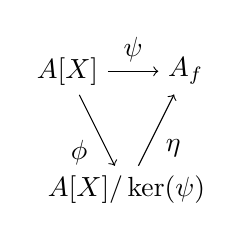
\begin{tikzpicture}[node distance=1.5cm, auto]
    \node (G)    {$A[X]$};
    \node (H) [right of=G] {$A_f$};
    \node (GmodK) [below of=G, xshift=0.75cm] {$A[X]/\ker(\psi)$};

    \draw[->] (G) to node {$\psi$} (H);
    \draw[->] (G) to node [swap] {$\phi$} (GmodK);
    \draw[->] (GmodK) to node [swap] {$\eta$} (H);
  \end{tikzpicture}

  Thus we want to prove that $ker(\psi) = (Xf-1)$, so that $\frac{A[X]}{ker(\psi)} = \frac{A[X]}{(Xf-1)}$, and the lemma is proven.

  \vspace{0.3cm}
  First, observe that $\psi(Xf-1) = \psi(X)\psi(f)-\psi(1) = \frac{1}{f} \frac{f}{1} - 1 = 1-1=0$,
  so $Xf-1 \in ker(\psi)$, ie. $(Xf-1) \subseteq ker(\psi)$.

  Now, we want to prove that $ker(\psi) \subseteq (Xf-1)$.

  Take $h \in ker(\psi)$, will prove that $h \in (Xf-1)~ \foracll~ h \in ker(\psi)$, and thus $ker(\psi) \subseteq(Xf-1)$.

  \vspace{0.3cm}
  Want to prove that $h(X)$ is a multiple of $(Xf-1)$.

  Let
  $$h(X)=a_n X^n + a_{n-1} X^{n-1} + \ldots + a_1 X + a_0$$

  % Since $h \in ker(\psi) ~~\Longrightarrow~~ \psi(h)=0$, so
  % $$\psi(h) = \frac{a_n}{f^n} + \frac{a_{n-1}}{f^{n-1}} + \ldots \frac{a_1}{f} + \frac{a_0}{1} = 0 \in A_f$$

  multiply $h(X)$ by $f^n$:
  $$f^n \cdot h(X)=a_n (f^n X^n) + a_{n-1} f (f^{n-1} X^{n-1}) + a_{n-2} f^2 (f^{n-2} X^{n-2})  \ldots$$

  Note that since $\forall~ i \geq 1,~~ f^i X^i = (Xf -1)\cdot (f^{i-1} X^{i-1} + f^{i-2} X^{i-2} + \ldots + 1)$, then $f^i X^i \equiv 1 \pmod{Xf-1}$.

  So,
  $$f^n \cdot h(X)=\underbrace{a_n (1) + a_{n-1} f (1) + a_{n-2} f^2 (1) + \ldots + a_0 f^n}_{C~~\text{(constant)}} \pmod{Xf-1}$$

  $$\Longrightarrow~~ f^n \cdot h(X)=C \pmod{Xf-1}$$
  $$\Longleftrightarrow~~ f^n \cdot h(X)=Q(X) \cdot (Xf-1) + C$$

  Want to remove $C$, but it is non-zero. Note that in $A_f$ (ring of fractions), $a\f^n = 0$ iff $\exist~ k$ such that $f^k \cdot a = 0$ in $A$.

  So, multiply both sides by $f^k$:
  $$f^k \cdot f^n \cdot h(X)=f^k \cdot (Q(X) \cdot (Xf-1) + C)$$
  $$\underbrace{f^k f^n}_{f^{nk}} \cdot h(X)=\underbrace{f^k Q(X)}_{Q'(X)} \cdot (Xf-1) + \underbrace{f^k C}_{0}$$

  $$\Longrightarrow~~ f^{n+k} \cdot h(X)=Q'(X) \cdot (Xf-1)$$
  $$\Longleftrightarrow~~ f^{n+k} \cdot h(X) \equiv 0 \pmod{Xf-1}$$

  multiply it by $X^{n+k}$:
  $$X^{n+k} \cdot f^{n+k} \cdot h(X) \equiv X^{n+k} \cdot 0 \pmod{Xf-1}$$
  $$(Xf)^{n+k} \cdot h(X) \equiv 0 \pmod{Xf-1}$$

  Now, since we had $Xf \equiv 1$ in $\frac{A[X]}{(Xf-1)}$,
  $$(1)^{n+k} \cdot h(X) \equiv 0 \pmod{Xf-1}$$
  $$\Longrightarrow~~ h(X) \equiv 0 \pmod{Xf-1}$$
  By definition this is saying $h(X) \in (Xf-1) ~\forall~ k \in ker(\psi)$.

  Thus $ker(\psi) \subseteq (Xf-1)$.

  Initially we saw that $(Xf-1) \subseteq ker(\psi)$. Therefore $ker(\psi)=(Xf-1)$.

  Hence,
  $$A_f \cong \frac{A[X]}{(Xf-1)}$$
\end{proof}



\newpage

\section{Exercises}

For the exercises, I follow the assignments listed at \cite{mit-course}.

The exercises that start with \textbf{R} are the ones from the book \cite{reid}, and the ones starting with \textbf{AM} are the ones from the book \cite{am}.

\subsection{Exercises Chapter 1}

\begin{ex}{R.1.1}
  Ring $A$ and ideals $I, J$ such that $I \cup J$ is not an ideal. What's the smallest ideal containing $I$ and $J$?
\end{ex}
\begin{proof}
  Take ring $A= \mathbb{Z}$. Set $I = 2 \mathbb{Z},~ J=3 \mathbb{Z}$.

  $I,~J$ are ideals of $A$ ($=\mathbb{Z}$). And $I \cup J = 2 \mathbb{Z} \cup 3 \mathbb{Z}$.\\
  Observe that for $2 \in I,~ 3 \in J ~\Longrightarrow~ 2,3 \in I \cup J$, but $2+3 = 5 \not\in I \cup J$.

  Thus $I \cup J$ is not closed under addition; thus is not an ideal.


  Smallest ideal of $\mathbb{Z}$ ($=A$) containing $I$ and $J$ is their sum:

  $$I+J = \{ a+b | a \in I, b \in J \}$$

  $gcd(2,3)=1$, so $I+J = \mathbb{Z}$.

  Therefore, smallest ideal containing $I$ and $J$ is the whole ring $\mathbb{Z}$.
\end{proof}

\begin{ex}{R.1.5}
  let $\psi: A \longrightarrow B$ a ring homomorphism. Prove that $\psi^{-1}$ takes prime ideals of $B$ to prime ideals of $A$.\\
  In particular if $A \subset B$ and $P$ a prime ideal of $B$, then $A \cap P$ is a prime ideal of $A$.
\end{ex}
\begin{proof}
  (Recall: prime ideal is if $a,b \in R$ and $a \cdot b \in P$ (with $R \neq P$), implies $a \in P$ or $b \in P$).

  Let
  $$\psi^{-1}(P) = \{ a \in A | \psi(a) \in P \} = A \cap P$$
  The claim is that $\psi^{-1}(P)$ is prime ideal of $A$.

  \begin{enumerate}[i.]
    \item show that $\psi^{-1}(P)$ is an ideal of $A$:\\
      $0_A \in \psi^{-1}(P)$, since $\psi(0_A)=0_B \in P$ (since every ideal contains $0$).

      If $a,b \in \psi^{-1}(P)$, then $\psi(a), \psi(b) \in P$, so
      $$\psi(a-b)= \psi(a) - \psi(b) \in P$$
      hence $a-b \in \psi^{-1}(P)$.

      If $a \in \psi^{-1}(P)$ and $r \in A$, then $\psi(ra) = \psi(r) \psi(a) \in P$, since $P$ is an ideal.\\
      Thus $ra \in \psi^{-1}(P)$.

      $\Longrightarrow$ so $\psi^{-1}$ is an ideal of $A$.

    \item show that $\psi^{-1}(P)$ is prime:\\
      $\psi^{-1}(P) \neq A$, since if $\psi^{-1}(P)=A$, then $1_A \in \psi^{-1}(P)$, so $\psi(1_A)=1_B \in P$, which would mean that $P=B$, a contradiction since $P$ is prime ideal of $B$.

      Take $a,b \in A$ with $ab \in \psi^{-1}(P)$; then $\psi(ab) \in P$, and since $\psi$ is a ring homomorphism, $\psi(ab) = \psi(a)\psi(b)$.

      Since $P$ prime ideal, then $\psi(a)\psi(b) \in P$ implies either $\psi(a) \in P$ or $\psi(b) \in P$.\\
      Thus $a \in \psi^{-1}(P)$ or $b \in \psi^{-1}(P)$.

      Hence $\psi^{-1}(P)$ ($=A \cap P$) is a prime ideal of $A$.
  \end{enumerate}
\end{proof}


\begin{ex}{R.1.6}
  prove or give a counter example:
  \begin{enumerate}[a.]
    \item the intersection of two prime ideals is prime
    \item the ideal $P_1+P_2$ generated by $2$ prime ideals $P_1,P_2$ is prime
    \item if $\psi: A \longrightarrow B$ ring homomorphism, then $\psi^{-1}$ takes maximal ideals of $B$ to maximal ideals of $A$
    \item the map $\psi^{-1}$ of Proposition 1.2 takes maximal ideals of $A/I$
      to maximal ideals of $A$
  \end{enumerate}
\end{ex}
\begin{proof}
  \begin{enumerate}[a.]
    \item let $I = 2 \mathbb{Z} = (2)$, $J = 3 \mathbb{Z} = (3)$ be ideals of $\mathbb{Z}$, both prime.

      Then $I \cap J = (2) \cap (3) = (6)$.

      The ideal $(6)$ is not prime in $\mathbb{Z}$, since $2 \cdot 3 \in (6)$, but $2 \neq (6)$ and $3 \neq (6)$.

      Thus the intersection of two primes can not be prime.

    \item $P_1=(2),~ P_2=(3)$, both prime.

      Then,
      $$P_1 + P_2 = (2)+(3)=\{ a+b | a \in P_1, b \in P_2 \}$$

      $\longrightarrow~$ in a principal ideal domain (like $\mathbb{Z}$), the sum of two principal ideals is again principal, and given by $(m)+(n)=(gcd(m,n))$.

      (recall: principal= generated by a single element)

      So, $P_1+P_2= (2)+(3) = (gcd(2,3))=(1)=\mathbb{Z}$.

      The whole ring is not a prime ideal (by the definition of the prime ideal), so $P_1+P_2$ is not a prime ideal.

      Henceforth, the sum of two prime ideals is not necessarily prime.

    \item let $A=\mathbb{Z},~ B=\mathbb{Q},~ \psi: A \longrightarrow B$.

      Since $\mathbb{Q}$ is a field, its only maximal ideal is $(0)$.

      Then
      \begin{align*}
        \psi^{-1}( (0) ) &= (0) \subset \mathbb{Z}\\
        \text{ie.}~ \psi^{-1}( m_B ) &= (m_B) \subset A
      \end{align*}

      But $(0)$ is not maximal in $\mathbb{Z}$, because $\mathbb{Z}/(0) \cong \mathbb{Z}$ is not a field.

      Thus the preimages of maximal ideals under arbitrary ring homomorphisms need not be maximal.

    \item $\psi: A \longrightarrow A/I$ quotient homomorphism, $I \subseteq A$ an ideal.

      Let $M$ a maximal ideal of $A/I$, then $\frac{(A/I)}{M}$ is a field (Proposition 1.3).

      By the isomorphism theorems,
      $$\frac{(A/I)}{M} \cong \frac{A}{\psi^{-1}(M)}$$


      Since $\frac{(A/I)}{M}$ is a field, the quotient $\frac{A}{\psi^{-1}(M)}$ is a field, so $\psi^{-1}(M)$ is a maximal ideal of $A$.

      $\Longrightarrow~$ under $\psi$, preimages of maximal ideals are maximal.
  \end{enumerate}
\end{proof}

\begin{ex}{R.1.12.a}
  if $I,J$ ideals and $P$ prime ideal, prove that
  $$IJ \subset P ~\Longleftrightarrow~ I \cap J \subset P ~\Longleftrightarrow~ I ~\text{or}~ J \subset P$$
\end{ex}
\begin{proof}
  assume $I \subseteq P$ (for $J \subseteq P$ will be the same, symmetric), take $x \in IJ$,

  then
  $$x = \sum_{k=1}^n a_k b_k$$
  with $a_k \in I,~ b_k \in J$.

  Each $a_k \in I \subseteq P$. Since $P$ an ideal,
  $$\sum_{k=1}^n a_k b_k \in P$$

  thus $x \in P$, hence $IJ \subseteq P$.

  So $I \subseteq P$ or $J \subseteq P$ $~\Longrightarrow IJ \subseteq P$.

  \vspace{0.5cm}
  Conversely,\\
  assume $P$ prime and $IJ \subseteq P$.

  Suppose by contradiction that $I \not\subseteq P$ and $J \not\subseteq P$.
  \begin{itemize}
    \item[-] since $I \not\subseteq P,~ \exists a \in I$ with $a \not\in P$
    \item[-] since $J \not\subseteq P,~ \exists b \in J$ with $b \not\in P$
  \end{itemize}
  Since $a \in I,~ b \in J,~~ ab \in IJ \subseteq P$, but $P$ is prime, so $ab \in P$ implies that $a \in P$ or $b \in P$. This contradicts $a,b$ being taken outside of $P$.

  Thus $I \not\subseteq P$ and $J \not\subseteq P$ are false.

  \vspace{0.3cm}
  So both directions are proven, hence
  $$IJ \subseteq P ~\Longrightarrow~ I \subseteq P ~\text{or}~ J \subseteq P$$

\end{proof}

\begin{ex}{R.1.18}
  Use Zorn's lemma to prove that any prime ideal $P$ contains a minimal prime ideal.
\end{ex}
\begin{proof}
  Let $P$ prime ideal of $R$.

  $$S = \{ Q \subseteq R ~|~ Q ~\text{a prime ideal AND}~ Q \subseteq P \}$$

  Goal: show that $S$ has a minimal element, the minimal ideal contained in $P$.

  $P \subset S$, so $S$ is nonempty.

  Let $C \subseteq S$ be a chain (= totally ordered subset) with respect to inclusion.

  Define
  $$Q_C = \bigcap_{Q \in C} Q$$

  Clearly $Q_C \subseteq P$, since each $Q \in C$ is $Q \subseteq P$.

  Since $C$ is ordered by inclusion, it is a decreasing chain of prime ideals.

  Intersection of a decreasing chain of prime ideals is again a prime ideal:
  \begin{itemize}
    \item[-] if $ab \in Q_C$, then $ab \in Q ~\forall Q \in C$
    \item[-] since $Q$ prime, $\forall Q \in C$ either $a \in Q$ or $b \in Q$
  \end{itemize}

  If there were some $Q_1,~ Q_2 \in C$ with $a \in Q_1$ and $b \not\in Q_2$, then by total ordering, either $Q_1 \subseteq Q_2$ or $Q_2 \subseteq Q_1$.

  In either case: contradiction, since the smaller one would have to contain the element that was assumed to be excluded.

  Thus $\forall Q \in C$ the same element $a, b$ must lie in all $Q$. $\Longrightarrow~$ lies in the intersection of them, $Q_C$.

  Henceforth, $Q_C$ is a prime ideal and lies in $S$, and its a lower bound of $C$ in $S$.

  Now, $S$ is nonempty, and every chain in $S$ has a lower bound in $S$ (its intersection).\\
  Therefore, $S$ has a minimal element $P_{min}$.

  By construction, $P_{min}$ is a prime ideal $P_{min} \subseteq P$, and by minimality there are no strictly smaller prime ideals inside $P$.

  So $P_{min}$ is a minimal prime ideal, contained in $P$.
\end{proof}

\begin{ex}{R.1.10}
\end{ex}
\begin{proof}
\end{proof}

\begin{ex}{R.1.11}
\end{ex}
\begin{proof}
\end{proof}

\begin{ex}{R.1.4}
\end{ex}
\begin{proof}
\end{proof}

\subsection{Exercises Chapter 2}

\begin{ex}{R.2.9}
$0 \longrightarrow L \stackrel{\alpha}{\longrightarrow} M \stackrel{\beta}{\longrightarrow} N \longrightarrow 0$ is a s.e.s. of $A$-modules. Prove that if $N, L$ are finite over $A$, then $M$ is finite over $A$.
\end{ex}
\begin{proof}
  Denote the generators of $L$ and $N$ respectively as
  \begin{align*}
    \{l_1, \ldots, l_k \} &\subseteq L\\
    \{n_1, \ldots, n_p \} &\subseteq N
  \end{align*}

  By s.e.s. definition, 
  \begin{itemize}
    \item[-] $\alpha$ is injective (one-to-one), so
    $$\forall l_i \in L,~ \exists~ x_i \in M ~\text{s.th.}~ \alpha(l_i)=x_i$$

  \item[-] $\beta$ is surjective (onto), so
    $$\forall n_j \in N,~ \exists~ y_j \in M ~\text{s.th.}~ \beta(y_j)=n_j$$
\end{itemize}

  We will show that $\{x_1, \ldots, x_k, y_1, \ldots, y_p \}$ generate $M$, and thus $M$ is finite:

  Let $m \in M$, then $\beta(m) \in N$, and
  $$\beta(m) = \sum_{j=1}^p a_j n_j ~~~\text{with}~ a_j \in A$$

  Take $m' \in M$, with $m' = \sum a_j y_j$, then
  $$\beta(m') = \sum a_j \beta(y_j) = \sum a_j n_j = \beta(m)$$

  Then, since $\beta(m)=\beta(m')~~ \Longrightarrow~~ \beta(m-m')=0$, thus
  $$(m-m') \in ker(\beta)$$

  By \emph{exactness} property, since $\alpha: L \longrightarrow ker(\beta)$, we have $ker(\beta)=im(\alpha)$.

  Therefore, $\exists~ l \in L$ such that $\alpha(l)= m-m'$.

  Since $\{l_i\}_k$ generate $L$,
  $$l = \sum^k b_i l_i$$
  thus
  $$m-m' = \alpha(l) = \alpha(\underbrace{\sum b_i l_i}_{l}) = \sum b_i \underbrace{\alpha(l_i)}_{x_i} = \sum b_i x_i$$

  Rearrange,
  $$m = m' + \sum b_i x_i = \sum_{j=1}^p a_j y_j + \sum_{i=1}^k b_i x_i ~~~~~ \forall m \in M$$

  So, $L$ provides $k$ generators for the kernel part of $M$, $N$ provides $p$ "lifts" for the quotient part of $M$; thus $M$ is generated by $k+p$ elements.\\
  Thus $M$ is finitely generated over $A$.
\end{proof}


\subsection{Exercises Chapter 3}

\begin{ex}{R.3.2}
  $K$ a field, $A \supset K$ a ring which is finite dimensional as a $K$-vector space.
   Prove that $A$ is Noetherian and Artinian.
\end{ex}
\begin{proof}
  $dim(A)=n < \infty$, so every ideal $\aA$ of $A$ is a $K$-subspace of $A$, because if $x \in \aA$ and $c \in K$, then $c \cdot x \in \aA$.

  \begin{enumerate}
    \item Noetherian:\\
      let $I_1 \subseteq I_2 \subseteq \ldots$ be an ascending chain of ideals in $A$.

      Since each $I_i$ is a subspace, we have
      $$dim_K(I_1) \leq dim_K(I_2) \leq \ldots \leq n$$
      where at some $i=m$ we have $dim_K(I_m)=dim_K(I_{m+1})$; then since $I_m \subseteq I_{m+1}$, we have $I_m = I_{m+1}$. So $A$ is Noetherian.
      
    \item Artinian:\\
      Similarly, if $I_1 \supseteq I_2 \supseteq \ldots$ a descending chain of ideals in $A$.

      then
      $$n \geq dim_K(I_1) \geq dim_K(I_2) \geq \ldots \geq 0$$
      where at some $i=m$ we have $dim_K(I_m)=dim_K(I_{m+1})$; then since $I_m \subseteq I_{m+1}$, we have $I_m = I_{m+1}$. So $A$ is Artinian.
  \end{enumerate}
\end{proof}

\begin{ex}{R.3.5}
  Let $0 \longrightarrow L \stackrel{\alpha}{\longrightarrow} M \stackrel{\beta}{\longrightarrow} N \longrightarrow 0$ an exact sequence. Let $M_1, M_2 \subseteq M$ be submodules of $M$.

  Prove if the following holds or not:
  $$\beta(M_1)=\beta(M_2) ~\text{and}~ \alpha^{-1}(M_1)=\alpha^{-1}(M_2)~~\Longrightarrow~ M_1=M_2$$
\end{ex}
\begin{proof}
  Counterexample showing that it does not hold:

  Let $K$ a field, $M = K \oplus K~, L=K,~N=K$.

  Set, for $l \in L,~ (m_1, m_2) \in M$,
  \begin{align*}
    \alpha:~ &l \longmapsto (l, 0)\\
    \beta:~ &(m_1, m_2) \longmapsto m_2
  \end{align*}

  So we have
  $$0 \longrightarrow K \stackrel{\alpha}{\longrightarrow} K^2 \stackrel{\beta}{\longrightarrow} K \longrightarrow 0$$

  Then,
  \begin{align*}
    M_1 &= \{ (x, x) ~|~ x \in K\} ~~~~\sim\text{(diagonal line)} \\
    M_2 &= \{ (0, x) ~|~ x \in K\} ~~~~\sim\text{(y-axis)}
  \end{align*}

  (Geometric interpretation: $M_1,~ M_2$ are the \emph{diagonal line} and \emph{y-axis} respectively; and $\alpha,~\beta$ capture information about the \emph{vertical} components (x-axis, y-axis respectively), but not about the \emph{diagonal} way a submodule is embedded in $M$).

  Then,
  \begin{align*}
    \beta(M_1) &= \{ x ~|~ x \in K\} = K \\
    \beta(M_2) &= \{ x ~|~ x \in K\} = K
  \end{align*}
  thus, $\beta(M_1) = \beta(M_2)$.

  For $M_1,~~ (l,0)\in M$ iff $l=0$, thus $\alpha^{-1}(M_1) = \{0\}$,\\
  for $M_2,~~ (l,0)\in M$ iff $l=0$, thus $\alpha^{-1}(M_2) = \{0\}$,\\
  thus $\alpha^{-1}(M_1)=\alpha^{-1}(M_2)$.


  So we've seen that
  \begin{align*}
    \beta(M_1) = \beta(M_2)\\
    \alpha^{-1}(M_1)=\alpha^{-1}(M_2)
  \end{align*}
  while having $M_1 \neq M_2$.
\end{proof}



\begin{ex}{R.3.3}
Let $A$ a ring, $I_1, \ldots, I_k$ ideals such that each $A/I_i$ is a Noetherian ring.
Prove that $\bigoplus A/I_i$ is a Noetherian $A$-module, and deduce that if $\bigcap I_i = 0$ then $A$ is also Noetherian.
\end{ex}
\begin{proof}
\begin{enumerate}[i.]
  \item by Corollary \ref{R.3.5} (i), if $M_i$ Noetherian modules, then $\bigoplus M_i$ is Noetherian.
    $\Longrightarrow$ thus $\bigoplus A/I_i$ is Noetherian.
  \item Take the canonical homomorphism
    $$\phi: A \longrightarrow \bigoplus_{i=1}^n A/ I_i$$
    by $\phi(a) = (a+I_1, a+I_2, \ldots, a+I_n)$.

    $\phi$ is injective: $ker(\phi)= \{ a \in A | a \in I_i \forall i \}$.

    Since we're given $\cap I_i = 0$, then $ker(\phi)=\cap I_i$, and $\phi$ is injective.

    Thus, $\phi$ is the isomorphism $A \cong im(\phi)$, where $im(\phi)$ is an $A$-submodule of $\bigoplus A/I_i$.

    We know that any submodule of a Noetherian module is Noetherian, thus, since
    \begin{itemize}
      \item $A/I_i$ is Noetherian by hypothesis of the exercise
      \item $A \cong im(\phi)$
      \item $im(\phi)$ is an $A$-submodule of $\bigoplus A/I_i$
  \end{itemize}
  then, $A$ is Noetherian.
\end{enumerate}
\end{proof}

\begin{ex}{R.3.4}
  Prove that if A is a Noetherian ring and M a finite A-module, then there
  exists an exact sequence $A^q \stackrel{\alpha}{\longrightarrow} A^p \stackrel{\beta}{\longrightarrow} M \longrightarrow 0$.
  That is, M has a presentation as an A-module in terms of finitely many generators and relations.
\end{ex}
\begin{proof}
  since $M$ fingen $~\Longrightarrow~$ generators $\{m_1, \ldots, m_2 \} \subseteq M$ span $M$.

  Let $\beta$ be a surjective $A$-linear map, which forms a free $A$-module of rank $p$ onto $M$:
  \begin{align*}
    \beta: A^p &\longrightarrow M\\
    (a_1, \ldots, a_p) &\longmapsto \sum_{i=1}^p a_i m_i
  \end{align*}

  Let $K=ker(\beta)$. By the 1st Isomorphism Theorem,
  $$M \cong A^p / K$$

  Since $A$ is a Noetherian ring, then every free $A$-module of finite rank (eg. $A^p$) is a Noetherian module.

  Every submodule of a Noetherian module is fingen.

  $\Longrightarrow~$ since $K \subseteq A^p, ~\Longrightarrow~ K ~~(=ker(\beta))$ is fingen.

  Since $K$ fingen, let $\{k_1, \ldots, l_q\}$ be generators of $K$.

  Define $\psi: A^q \longrightarrow K$.

  Compose it with the inclusion map $i: K \longrightarrow A^p$,
  $$\alpha = i \circ \psi:~ A^q \longrightarrow A^p$$

  So we have the whole sequence $A^q \stackrel{\alpha}{\longrightarrow} A^p \stackrel{\beta}{\longrightarrow} M \longrightarrow 0$, where
  \begin{itemize}
    \item $\beta$ is surjective
    \item $im(\alpha)=ker(\beta)$
  \end{itemize}
  so that it is a exact sequence, thus, $M$ has a finite presentation.
\end{proof}

\subsection{Exercises Chapter 4}

\begin{ex}{R.4.1.a}
  $k[X^2] \subset k[X]$ is a finite extension, hence integral. Find the integral dependence relation for any $f \in k[X]$.
\end{ex}
\begin{proof}
  $\forall f(X) \in k[X]$ can be uniquely decomposed into its even and odd parts:
  $$f(X) = p(X^2) + X \cdot q(X^2)$$

  with $p(X^2),~ q(X^2) \in k[X^2]$, and\\
  $p(X^2)$: sum of all terms with even exponents\\
  $q(X^2)$: sum of all terms with odd exponents, and then factoring out $X$.

  \vspace{0.3cm}
  (Observation: this is used in FRI cryptographic protocol\\
  \href{https://github.com/arnaucube/math/blob/master/notes_fri_stir.pdf}{https://github.com/arnaucube/math/blob/master/notes\_fri\_stir.pdf})


  Rearrange it
  \begin{align*}
    f(X) &- p(X^2) = X \cdot q(X^2), ~~\text{square:}\\
    (f(X) &- p(X^2))^2 = X^2 \cdot q(X^2)^2\\
    f(X)^2-2 p(X^2) f(X) &+ p(X^2)^2 = X^2 \cdot q(X^2)^2\\
    f(X)^2 \underbrace{-[2 p(X^2)]}_{a_1} f(X) &+ \underbrace{[p(X^2)^2 - X^2 \cdot q(X^2)^2]}_{a_0} = 0
  \end{align*}

   Denote the last polynomial as $P(T) \in k[X^2]$, where $f(X)$ is a root of $P(T)$.

   \vspace{0.2cm}
   The integral dependence relation for any $f \in k[X]$ is given by the monic polynomial from \ref{R.4.1}.ii, in this case $T^2 + a_1 T + a_0 = 0$ with $a_i \in k[X^2]$.

   We have that
   \begin{align*}
     a_1 &= -2 p(X^2)\\
     a_0 &= p(X^2)^2 - X^2 q(X^2)^2
   \end{align*}


   So for example, for $f(X)= X^3 + X^2 + X + 1$:
   \begin{align*}
     f(X) = (X^2 + 1) &+ X (X^2 + 1)\\
     (f(X) - (X^2+1))^2 &= X^2 (X^2 + 1)^2\\
     (f(X) - p(X))^2 &= X^2 (q(X))^2
   \end{align*}
\end{proof}


\begin{ex}{R.4.5}
  Let $A=k[X,Y]/(Y^2 - X^2 - X^3)$. Prove that the normalization of $A$ is $k[t]$ where $t=Y/X$.
\end{ex}
\begin{proof}
$A=k[X,Y]/(Y^2 - X^2 - X^3)$, express $X$ and $Y$ in terms of $t$:

Since $t=Y/X$ then $Y=tX$, and combined with $Y^2 = X^2 + X^3$, then
\begin{align*}
  (tX)^2 &= X^2 + X^3\\
  t^2 X^2 &= X^2 + X^3, ~~\text{assuming}~X \neq 0:\\
  t^2 &= 1+X, ~\text{thus}\\
  X&=t^2-1 \in k[X]
\end{align*}

Then, $Y=tX=t(t^2-1)=t^3-t \in k[X]$.

Hence $X, Y \in k[X]$.

Therefore, $k[X,Y]/(Y^2 - X^2 - X^3) \subseteq k[t]$.

\vspace{0.4cm}
By \ref{noether-normalization} (Noether normalization lemma), to show that $k[t]$ is the \emph{normalization}, must show that $k[t]$ is \emph{integral} over $A$.

From $X=t^2-1 ~~\Longrightarrow~~ t^2-1-X=0 ~~\Longrightarrow~ t^2 - (1+X) = 0$.

$(1+X) \in A$, so $t$ satisfies the monic polynomial
$$P(T) = T^2 - (1+X) \in A[T]$$
Thus $t$ is integral over $A$.

Since $k[t]$ is generated by $t$ over $k$, and $k \subset A$, then the entire ring $k[t]$ is integral over $A$.

Since $k[t]$ is a polynomial ring over a field, which is a UFD, it is integrally closed (since all UFD are integrally closed).

$Frac A = k(X,Y)$, since $X=t^2-1, ~Y=t^3-t ~~\Longrightarrow~ k(X,Y) \subseteq k(t)$

and $t=Y/X \in k(X,Y)$, thus $k(X,Y)=k(t)$.

Since $k[t]$ is integrally closed and is the integral closure of $A$ in its fraction field $k(t)$, we conclude that the normalization of $A$ is $k[t]$.
\end{proof}



\begin{ex}{R.4.9}
  $k$ a field, $A= k[X,Y,Z]/(X^2- Y^3 -1, XZ - 1)$, find $\alpha, \beta \in k$ such that $A$ is integral over $B = k[X + \alpha Y + \beta z]$, and write a set of generators of $A$ as a $B$-module.
\end{ex}
\begin{proof}
  (want to find a linear combination of the coordinates such that the original variables satisfy monic polynomials over the new ring $B$)

  The relations defining $A$ are
  \begin{align*}
    X^2-Y^3-1=0 ~~&\Longrightarrow~ Y^3 = X^2 -1 ~~~(*)\\
    XZ -1=0 ~~&\Longrightarrow~ Z= 1/X = X^{-1}
  \end{align*}

Thus $A$ can be denoted as $A = k[X,Y,X^{-1}]/(Y^3 - X^2 - 1)$.


Now, $Y$ is inegral over $k[X]$, since $Y^3 - (X^2 - 1) = 0$ is monic in $Y$ with coefficients in $k[X]$.

$Z$ is not integral over $k[X]$, since $Z=1/X$ and $X$ is not a unit in $k[X]$.

Choose $\alpha, \beta \in k$ such that $X$ (and thus $Z$) becomes integral over $B$:\\
set $\alpha=0,~\beta=1 ~~\Longrightarrow~~ B=k[X+\alpha Y + \beta Z]= k[X+Z]$.

Let $w=X+Z$; since $XZ=1$, we have
$$w=X+\frac{1}{X} ~~\Longrightarrow~~ Xw=X^2+1 ~~\Longrightarrow~~ X^2 -w X +1 = 0 ~~(**)$$

which is monic with coefficients in $k[w]$, thus $X$ is integral over $B$.

Since $Z=w-X$, $Z$ is also integral.

\vspace{0.4cm}
Generators of $A$ as a $B$-module:

we hadd $B=k[w]$ with $w=X+Z$.

From $(**)$ we have $X^2 - wX + 1=0$, so $X^2 = wX -1$.

Thus any polynomial in $X$ can be reduced to a linear form $b_1 X + b_0$ with $b_i \in k[w]$. Hence it's partial basis is $\{1, X\}$.

Fitting $X^2$ into $(*)$,
\begin{align*}
  X^2 &- Y^3 -1 =0\\
  Y^3 &= X^2-1\\
  Y^3 &= wX -2
\end{align*}

thus any power of $Y$ higher than $2$ can be reduced (eg. $Y^4 = Y(wX-2) = w(XY) - 2Y$).

So its partial basis is $\{1, Y, Y^2\}$.

For $Z$, since $XZ=1$ and $w=X+Z \Longrightarrow Z=w-X$, thus $Z$ is a $B$-linear combination of $\{1,X\}$.

\vspace{0.2cm}
Combining the previous partial basis, the generators are
$$\{ 1, X \} \times \{ 1,Y, Y^2 \} = \{ 1, Y, Y^2, X, XY, XY^2 \}$$

\end{proof}

\bibliographystyle{unsrt}
\bibliography{commutative-algebra-notes.bib}

\end{document}
